\documentclass{seal_thesis}
\usepackage{caption}
\usepackage{subcaption}
\usepackage{float}
\usepackage[table,xcdraw]{xcolor}
\usepackage{multirow}
\usepackage{lscape}
\usepackage{graphicx}
\usepackage{tabularx}
\usepackage{longtable}
\usepackage[inline]{enumitem}
\usepackage{booktabs}



\thesisType{Bachelor Thesis}
\date{\today}
\title{A Correlation Analysis Involving Benchmark Stability and Source Code Features}

\author{Mikael Basmaci}
\home{Istanbul} % Geburtsort
\country{Turkey}
\legi{15-721-244}
\prof{Prof. Dr. Harald C. Gall}
\assistent{Christoph Laaber}
\email{mikael.basmaci@uzh.ch}
\url{<url if available>}
\begindate{25.03.2019}
\enddate{25.09.2019}

\begin{document}
\maketitle

\frontmatter

\begin{acknowledgements}
	Here comes the acknowledgements.
\end{acknowledgements}

\begin{abstract}
	Here comes the abstract.
\end{abstract}

\begin{zusammenfassung}
	Here comes the summary.
\end{zusammenfassung}

\tableofcontents
\listoffigures
\listoftables
\lstlistoflistings

\mainmatter

\chapter{Introduction}


Performance is one of the crucial qualities of a software system \cite{Woodside:2007:FSP:1253532.1254717}, and it shapes the way developers build elements of the software. It is affected by lots of factors such as the software itself, the operating system the software is run on, the middleware, the hardware or even the underlying communication networks\cite{Woodside:2007:FSP:1253532.1254717}. Better performance is important for many reasons. With better performance, a data driven application  will load the data faster, a calculation will result quicker, or an interactive software will be more responsive. All these examples show that more or same amount of work can be done in less time, with better performance. Being an important software quality factor, it can also play a big role on the profitableness of a company\cite{Nguyen:2014:ICS:2597073.2597092}\cite{costa2019}.\\
\\
Having a performant system nowadays is not only the wish of customers or stakeholders but also one of the goals of software developers when developing software. Till late 2000s, there has not been a lot of research on the field of software performance testing\cite{weyuker2000experience}. With the evolution of software engineering over the years and the constantly advancing technology that drives software engineering further, the importance of performance has grown. However, the primary problems encountered in the field of software engineering are often related to performance regressions\cite{weyuker2000experience}.\\
\\
A performance regression is to be found when a new version of the software gives a worse user experience in terms of performance, such as having longer response times, or consuming extra resources such as RAM or CPU while giving the same user experience\cite{Nguyen:2014:ICS:2597073.2597092}. Solutions to these kinds of problems include supply of more hardware, which comes costly and is not applicable for large software systems \cite{Nguyen:2014:ICS:2597073.2597092} or finding out the regression causes in the software by testing.\\
\\
To assess the performance of the system and improve it, Software Performance Engineering (SPE) activites are needed \cite{Woodside:2007:FSP:1253532.1254717}. There are two general approaches found in the literature: first one is called measurement-based SPE, which stands for experimental performance calculations made on the software to report about the performance, second one is called model-based, which refers to creating performance models while developing to meet the performance requirements\cite{Woodside:2007:FSP:1253532.1254717}. \\ 
\\
There are different kinds of performance testing belonging to measurement-based SPE found in the literature. One of them is stress testing, which tests the software system for the stability while putting it under extreme workloads to detect its breaking point. The longer the system holds, the more stable the system is. Another type of performance test is load testing, which tests the software system with high loads to find out about performance bottlenecks. These types of performance tests are useful for when one wants to assess the general performance of a complete software system before it goes into production. They are, however, quite complex in terms of setups, manual configurations and mostly important, having long execution times \cite{Nguyen:2014:ICS:2597073.2597092}. This complexity makes it hard to find performance regressions as fast as possible, causing delay in Continuos Deployment (CD) architectures \cite{Laaber:2018:EOS:3196398.3196407}.\\
\\
There exist another type of performance testing, which is with the so called software microbenchmarks. These are adopted as performance evaluation strategy for rather small and library-like projects\cite{laaber2019software} and can test modular functions of a software system and measure their performance\cite{costa2019}. With early adoption of these tests, developers can find out about performance regressions whilst developing, and find solutions before they become bigger performance issues, which one would first realize at the time of analyzing results of bigger performance tests such as stress or load tests. A challenge with testing using microbenchmarks is the non-deterministicity of the results, which means a certain variability exist for the results of an executed benchmark\cite{Laaber:2018:EOS:3196398.3196407}. A benchmark is said to be stable or not stable depending on the variability of its results. Having a stable benchmark is important because being stable means having less varying results across multiple executions, and the less variable the benchmark's results, the more accurate the benchmark is able to report about performance counters. This also indicates that developers can rely on the results of a stable benchmark with less questioning about their validity. There are multiple factors that affect the variability of a benchmark such as the platform where the benchmarks are executed, the hardware that executes them, or the programming language of the benchmark itself \cite{laaber2018performance}. One of the factors that might be affecting the variability of benchmarks could be the source code related features of a benchmark and it is therefore needed to study the correlation between source code features and the stability of a benchmark.\\
\\
In this thesis, I am studying the stability of benchmarks from 230 open source software projects written in Go. For this, I firstly analyze the variability of 4802 benchmarks across all projects from a given dataset which has benchmark results of the projects. Secondly, I extract source code features of these benchmarks by parsing their source code and doing a callgraph analysis. The source code features extracted in this thesis fall into two categories: (i) Language related source code features, which include syntactic aspects of the programming language such as loops, collections and similar, and (ii) standard library related features, with which indications about the usage of hardware and network related aspects such as I/O, http calls, and similar can be made. Thirdly, I do an analysis using the variability results of benchmarks and their source code features to assess the correlation between the stability of benchmarks and their source code features.\\
\\
To this end, I answer the following research questions: 

\begin{itemize}
	\item \textbf{RQ1: How stable are microbenchmark results of Go projects?}
\end{itemize}

\noindent My hypothesis for the the first research question is: I expect the benchmarks to have different percentages of variability values, having a normalized distribution between 1\% to 100\%. To answer my first research question, I get all the projects benchmarks, calculate their variability with different measurement metrics such as Coefficient of Variation (CV) and Relative Confidence Interval Width (RCIW), and report the variabilities of benchmarks for 228 valid projects, having in total valid 4589 benchmarks.\\
\\
\begin{itemize}
	\item \textbf{RQ2: Which source code properties contribute to the stability of benchmark results and how?}
\end{itemize}

\noindent My hypothesis for the second research question is: I expect to see significant effects of body related features and Go's standard library usages to the stability of benchmark results. In particular, I suppose that cyclomatic complexity, file IO, http calls and loops have a significant impact on the variability. For the second research question, I download all the projects from Github. Then I run my parser program Prophunt which collects the source code properties from all the functions and make a callgraph analysis for the benchmarks to collect all the visited functions' properties, resulting into properties of the benchmark. Finally, I use Spearman's rank-order correlation to find out about the correlation between extracted source code properties and the stability of a benchmark.\\
\\
Rest of this thesis is structured as follows: I give an introduction to related topics and background about this thesis in the \ref{Background and Related Work}. Chapter. In the \ref{Methodology}. Chapter, I explain the three steps I take to do the analytic part of this thesis and elaborate on the threads to the validity of the methodology. I present the results of these steps in the \ref{Results}. Chapter. Next comes the \ref{Discussion}. Chapter where I discuss about the methodology and the results of this thesis and present some ideas for the future work. I conclude with the \ref{Conclusion}. Chapter.

\chapter{Background and Related Work}
\label{Background and Related Work}

\section{Background}

In this subsection, I give a detailed background information about software microbenchmarks, their variability, the programming language Go and the way microbenchmarks are implemented and used in Go projects.

\subsection{Software microbenchmarks}

Different kinds of benchmarks are found in the literature. While sometimes benchmarks refer to a standardization of a measure, other benchmarks assess the performance of the underlying system. For example, there are different benchmark programs to measure the performance of hardware such as Central Processing Unit(CPU), to be able to compare their performance with others of its kind. Another example can be the benchmark function of a game, which gives the average Frames Per Second (FPS) score of the game run on a hardware.\\
\\
Software developers can analyze the performance of parts of their software with so called software microbenchmarks, which are found either as microbenchmarks or performance unit tests in the literature\cite{costa2019}. These two terms differ in the way they test the underlying code for performance: While microbenchmarks report performance counters (e.g., execution time, throughput, latency etc.) for the different iterations of a trial, performance unit tests act like unit tests in functional testing, reporting if a pre set performance criteria has been reached at the runtime of the test \cite{costa2019}. Some studies such as \cite{Stefan:2017:UTP:3030207.3030226}\cite{Horky:2015:UPU:2668930.2688051} investigate the usage of performance unit tests, while sometimes other studies such as \cite{Laaber:2018:EOS:3196398.3196407}\cite{rodriguez2016automatic} work with microbenchmarks. In this thesis, I work with microbenchmarks and in the rest of this thesis I use the term performance test interchangable with testing with microbenchmarks.\\
\\
Microbenchmarks usually test for only a small fraction of the software, such as one or multiple functions, to assess their performance. A microbenchmark can for instance test the performance of a newly introduced data structure, an implemented algorithm, or even the concurrency performance of functions\cite{costa2019}. As in functional testing, microbenchmarking also comes with testing frameworks that allow developers to create function pools, which are often also called microbenchmark suites (in contrast to unit test suites in functional testing). As an example, for Java there exist Java Microbenchmarking Harness (JMH), which is similar to JUnit, but is implemented to help developers with the creation of microbenchmarks\cite{JMH}.\\
\\
Go comes with a built-in package for testing and benchmarking, which makes it easier for developers to unit test their code while still developing, or measure the performance of their functions\cite{gobench}. To create a benchmark function, the only thing one has to write is a function beginning with the name \textbf{"Benchmark"} and give a parameter \textbf{*testing.B}. These functions are defined in files ending with the \textbf{\_test.go} suffix, and the collection of all the benchmarks within a project build its microbenchmarking suite. Listing \ref{BenchmarkSrc} shows the example benchmark \textit{BenchmarkHash} from project \textbf{ironsmile/nedomi} \cite{ironsmile/nedomi}.

\begin{lstlisting}[caption=An example benchmark from \cite{ironsmile/nedomi}., label={BenchmarkSrc}, language=Go, frame=single, breaklines=false]
func BenchmarkHash(b *testing.B) {
	var m = buildMapHash(id, count)
	for i := 0; b.N > i; i++ {
		if _, ok := m[first.Hash()]; !ok {
			b.Fail()
		}
		if _, ok := m[middle.Hash()]; !ok {
			b.Fail()
		}
		if _, ok := m[last.Hash()]; !ok {
			b.Fail()
		}
	}
}
\end{lstlisting}

\noindent A benchmark in Go can be executed by using the built-in command "go test" followed by a flag "-bench", and the benchmark invokes the target code b.N times \cite{gobench}. The default execution time of a benchmark is 1 second and the result of the benchmark is the average execution time of the target code across all runs. In this thesis, a full run of a benchmark is defined as iteration and the number of runs for a benchmark can be configured with a command-line flag "-count". The results of a benchmark refer to the collection of results from all iterations.\\
\\
Go developers can choose to run a benchmark for a limited time to see how many iterations can happen in this pre defined time, or also choose to run the benchmark for a specific amount of iterations to see how long it takes the functions within the benchmark to result in average. Such configurations are especially useful for when determining whether a new introduced feature in the system causes performance regressions. Furthermore, these regressions can be detected early whilst still being in the development stage of the software, and according changes to the code can be scheduled before the changes go to production, which ensures the stability for the performance in the evolution of the software.


\subsection{Microbenchmark variability}
\label{Microbenchmark variability}

Unless otherwise configured, when a microbenchmark is run, it executes the underlying code for a certain time period (e.g., 1s) over and over for each benchmark iteration and returns a collection of average execution times for each benchmark iteration\cite{laaber2019software}. Execution times of a benchmark in Go are expressed in nanoseconds \cite{laaber2019software} \cite{costa2019}. In this thesis, the term microbenchmark variability refers to the variability of a microbenchmark's resulting collection of execution times. It is basically computed by measuring how far the single execution times fall from the average execution time. In this manner, if the executions times are in the close neighborhood of the average value, the benchmark is considered as stable and it's predicted that another execution would take same or similar amount of nanoseconds as the average value. If, however, the points are distributed on a broader scale, it means that the benchmark is rather unstable, i.e., it cannot be predicted how long another execution of the benchmark will take.\\
\\
There are 2 main metrics that I use to calculate the variability of a microbenchmark in this thesis. The first one is called \textbf{coefficient of variation (CV)}, which is also known as the relative standard deviation\cite{laaber2019software}. "CV is a statistical measure for dispersion among a population of values" \cite{laaber2019software}, and in this thesis I use CV on the performance counters (i.e. average execution times in nanoseconds) of a microbenchmark's benchmark iterations to calculate the variation of a microbenchmark. CV is a measurement that is used to determine the variability in pervious studies as well \cite{laaber2019software} \cite{Leitner:2016:PCS:2926746.2885497}. Since CV expects the values to be on the same relative scale (ratio), it is not a statistically sound metric for performance data, because the the execution times of iterations do not form a normal distribution. Additionally, I calculate the \textbf{relative confidence interval width (RCIW)} with 95 and 99 percent confidence intervals of each microbenchmark and refer to them as RCIW95 and RCIW99 respectively. "The RCIW describes the estimated spread of the population's CV, as computed by statistical simulation"\cite{laaber2019software}.\\
\\
Regarding calculations of these metrics: CV is calculated by dividing the standard deviation of a dataset by the mean of the dataset. For RCIW, another methodology is followed, which is explained as bootstrapping with hierarchical random resampling with replacement and is also used in Laaber et al.'s paper \cite{laaber2019software}\cite{davison_hinkley_1997}\cite{hierach_data_2010} . The reason to follow this methodology resides in the non-normalized performance measurements \cite{laaber2019software}. Bootstrapping with randomly resampling refers to randomly sampling data points from a dataset, and in this thesis I use this technique with 10000 bootstraps on the execution times of each microbenchmark to generate a collection of normalized mean values out of them, which I can then use to create the 95 and 99 percent relative confidence intervals.

\begin{figure}[H]
	\centering
	\begin{subfigure}{.5\textwidth}
		\centering
		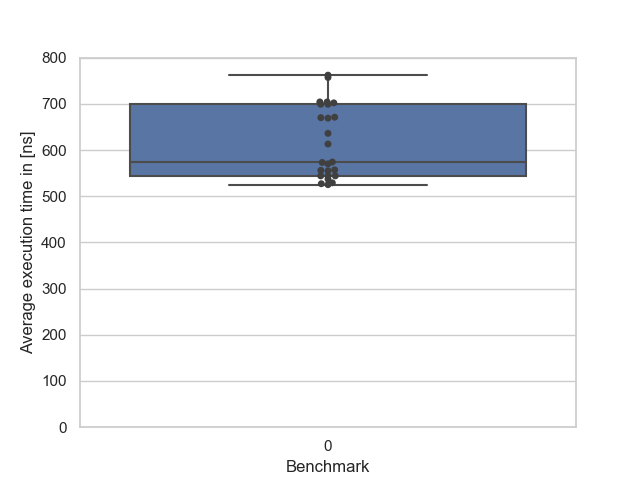
\includegraphics[width=\linewidth]{10percentvariance}
		\caption{Execution results of a microbenchmark with a RCIW99 of 10.06\%.}
		\label{fig:10percentvariance}
	\end{subfigure}%
	\begin{subfigure}{.5\textwidth}
		\centering
		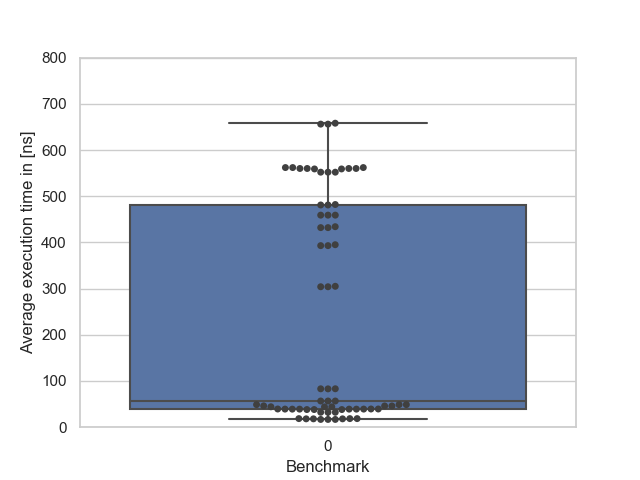
\includegraphics[width=\linewidth]{53percentvariance}
		\caption{Execution results of a microbenchmark with a RCIW99 of 53.41\%.}
		\label{fig:53percentvariance}
	\end{subfigure}
	\caption{Example for a low and high variance microbenchmark.}
	\label{fig:variances}
\end{figure}

\noindent To illustrate a low and high variable microbenchmark: Figure \ref{fig:10percentvariance} shows the execution times of the benchmark \textit{BenchmarkSerializeStruct} from \textbf{hprose/hprose-golang} project\cite{hprose/hprose-golang}. As the box plot shows, the points are all within the whiskers and close to the mean. Also, the distribution of the points vary from 525 to 762 nanoseconds and it has a 99 percent confidence interval width (RCIW99) of 10.06\%. In Figure \ref{fig:53percentvariance}, the benchmark \textit{BenchmarkEncoder} from \textbf{segmentio/objconv} project \cite{segmentio/objconv} is shown with its execution times. This benchmark's average execution times vary from 16.8 nanoseconds to 658 nanoseconds. This time, RCIW99 is 53.41\%. The  score in RCIW99 is an estimator for the variability, hence, the higher this score, the higher variability the benchmark has.\\
\\
The variability of a benchmark may depend on many factors such as the execution platform, the hardware the benchmarks are executed on, or, even the programming language of the microbenchmark itself\cite{laaber2018performance}. For example, the same benchmark can deliver different average values on different CPUs, as one CPU may perform much more operations in a second than the other one. Similarly, the same benchmark can have a different average for the execution time in a personal computer than the average in a cloud-based machine, or in different cloud-based machines compared to each other \cite{laaber2019software}. Some other factors include the concurrency, I/O latencies, virtualization etc \cite{laaber2019software}. \\
\\
Variability is a crucial factor of a benchmark, because it has an impact on the stability and reliability of it's results \cite{Laaber:2018:EOS:3196398.3196407}. It is important to have stable and reliable benchmarks, because then the developers can rely on the results of the microbenchmarks when they test parts of the software and find the regression causes with a higher trust. Therefore, it is essential to predict the stability of microbenchmarks. There has been studies trying to predict the variability of performance tests in public Infrastructure-as-a-Service (IaaS) clouds by comparing aspects such as hardware heterogeneity, multi-tenancy and control over optimizations \cite{Leitner:2016:PCS:2926746.2885497}, or by comparing the outcomes of forks, trials and iterations in terms of variability \cite{laaber2019software}. One way to predict the variability might be through analyzing source code properties of the software. This can on one hand help the developers identify the cause of slowdowns in a newer version for example, on the other hand help them understand which source code property affects the results in which way.\\
\\
Executing system-wide performance tests (e.g., stress tests, load tests etc.) of a software is usually a long, time consuming process that can take up to days to finish\cite{Laaber:2018:EOS:3196398.3196407}. If a developer can rely on the microbenchmarks of the software, this could help finding regression causing functions, but, it is still unknown whether microbenchmarks could replace system-wide performance tests in terms of finding performance regressions. When testing the software for performance via microbenchmarks, the aim of the developer is to have the highest possible coverage  with the minimal effort. For this, the minimal benchmark suite is needed, which should cover all or the most of the functionalities in the software. As the size of the software grows, the microbenchmark suite grows as well, and it gets harder to keep track of the tested and not tested functions. To this manner, the importance of predicting variability causes dives in. To keep the size of the benchmark suite minimal while having a good coverage, developers might not need testing all the functionalities. That's why, it's a good idea to predict which parts of the source code should be tested by predicting the variability of the benchmarks based on source code. With this, developers can be supported to write better benchmarks by for example being alerted to which new functions should have priorization in testing for performance.\\
\\
In this thesis, my aim is to find whether there is a correlation between the source code and the variability of a benchmark. For this, I analyze source code features of microbenchmarks written in Go and use them as dependent variables of a statistical equation,  where the independent variable is the variability of the benchmark in RCIW99. The results can be used to understand the correlation between source code and variability, as well as be used to predict the variability of a benchmark for further applications.\\

\subsection{Go}

Go is a statically typed, compiled programming language, designed at Google and was released in November 2009 \cite{go}. Some of its innovational features include built-in data structures for advanced concurrent programming, Goroutines as lightweight processes and built-in performance benchmarking/testing libraries. While still being quite a new language among other languages, Go is the forth most active programming language in Github, and third-most highly paid language globally, according to Stack Overflow Developer Survey 2019\cite{stackoverflowdev}. Furthermore, it is effectively used in the industry and has a growing community.\\
\\
An example run of a microbenchmark suite from \textbf{tidwall/buntdb} \cite{tidwall/buntdb} can be seen in Listing \ref{testbench}. The first column is the name of the benchmark, the second column is the amount of executions and the third column is the execution time per execution \cite{gobench}.
\begin{lstlisting}[caption=Example microbenchmark suite execution from \cite{tidwall/buntdb}., label={testbench}, frame=single, breaklines=false]
mikael@mikael-VirtualBox:~/Desktop/BenchmarkProjects/tidwall/buntdb/src-
/github.com/tidwall/buntdb$ go test -bench=.
goos: linux
goarch: amd64
pkg: github.com/tidwall/buntdb
Benchmark_Set_Persist_Random_1-4           	  300000	      4467 ns/op
Benchmark_Set_Persist_Random_10-4          	 1000000	      2094 ns/op
Benchmark_Set_Persist_Random_100-4         	 1000000	      1690 ns/op
Benchmark_Set_Persist_Sequential_1-4       	  500000	      3614 ns/op
Benchmark_Set_Persist_Sequential_10-4      	 1000000	      1388 ns/op
Benchmark_Set_Persist_Sequential_100-4     	 1000000	      1209 ns/op
Benchmark_Set_NoPersist_Random_1-4         	 1000000	      1774 ns/op
Benchmark_Set_NoPersist_Random_10-4        	 1000000	      1135 ns/op
Benchmark_Set_NoPersist_Random_100-4       	 1000000	      1107 ns/op
Benchmark_Set_NoPersist_Sequential_1-4     	 1000000	      1821 ns/op
Benchmark_Set_NoPersist_Sequential_10-4    	 2000000	       744 ns/op
Benchmark_Set_NoPersist_Sequential_100-4   	 2000000	       746 ns/op
Benchmark_Get_1-4                          	 2000000	       808 ns/op
Benchmark_Get_10-4                         	 3000000	       544 ns/op
Benchmark_Get_100-4                        	 3000000	       525 ns/op
Benchmark_Ascend_1-4                       	 5000000	       317 ns/op
Benchmark_Ascend_10-4                      	 2000000	       594 ns/op
Benchmark_Ascend_100-4                     	  500000	      3034 ns/op
Benchmark_Ascend_1000-4                    	   50000	     27257 ns/op
Benchmark_Ascend_10000-4                   	    5000	    271873 ns/op
Benchmark_Descend_1-4                      	 5000000	       304 ns/op
Benchmark_Descend_10-4                     	 3000000	       565 ns/op
Benchmark_Descend_100-4                    	  500000	      3065 ns/op
Benchmark_Descend_1000-4                   	   50000	     27362 ns/op
Benchmark_Descend_10000-4                  	    5000	    275479 ns/op
PASS
ok  	github.com/tidwall/buntdb	71.590s
\end{lstlisting}










\section{Related Work}

Performance testing, microbenchmarking and identifying performance regression causes are some of the prevalent topics in the field of Software Performance Engineering \cite{laaber2019software, Laaber:2018:EOS:3196398.3196407, costa2019, chenshang, Nguyen:2014:ICS:2597073.2597092, Luo, Alcocer:2015:TDP:2816707.2816718, Stefan:2017:UTP:3030207.3030226, Horky:2015:UPU:2668930.2688051, Leitner:2017:ESS:3030207.3030213}. Another extensive study field is analyzing performance variability of and within the production clouds \cite{Iosup, Leitner:2016:PCS:2926746.2885497}.\\
\\
To the best of my knowledge, there exist no study analyzing stability of software microbechmarks written in Go by trying to find a correlation with the underlying source code properties in these benchmarks. Furthermore, at the time of writing this thesis, most of the existing work is on the research of performance unit testing or microbenchmarking in the Java ecosystem \cite{Stefan:2017:UTP:3030207.3030226, Horky:2015:UPU:2668930.2688051, Leitner:2017:ESS:3030207.3030213, costa2019}, as also similarly stated in Stefan et al.'s paper \cite{Stefan:2017:UTP:3030207.3030226}. However, although being a fairly new language (introduction goes back to 2009), Go has become more popular in recent years and has taken its place in the research of software performance testing \cite{laaber2019software, Laaber:2018:EOS:3196398.3196407}.\\
\\
Laaber et al. report about the variability of microbenchmark results in various cloud environments \cite{laaber2019software}. For their study, they use 19 microbenchmarks from 4 open source projects, 2 of them being written with Java and the other 2 with Go. To analyze the stability of these benchmarks, they pick 3 well known Infrastructure as a Service (IaaS) providers and 1 bare-metal instance from IBM. From the 4.5 million unique microbenchmarking data points that they obtain from the executions in these environments, they show that the variation of benchmarks' CVs range from 0.03\% to over 100 \%. It is stated that the bare-metal instance's results are very stable, nearly followed by Amazon's Amazon Web Services (AWS) cloud. Google's Google Compute Engine (GCE) and Microsoft's Azure on the other hand do not retrieve reliable results. As a second research topic, they cast about the slowdown detectability of benchmarks and report that while low number of instances and trials cause high false-positive rates in detecting slowdowns, an increase of instances and trials affects slowdown detection rates positively. In a second paper by Laaber and Leitner \cite{Laaber:2018:EOS:3196398.3196407}, the research topic is the quality of the microbenchmark suite, which is investigated by studying 10 different OSS projects. In this study they analyze 5 Go and 5 Java projects' benchmarks suites and describe the size of benchmark suites, having 16 to 983 individual benchmarks and total execution times ranging from 11 minutes to 8.75 hours. To compare the stability of microbenchmarks, they use GCE and a self-managed bare-metal server. Their \textit{maxSpread} analysis shows that Go's benchmarks are very stable, mostly having a \textit{maxSpread} below 0.05 in bare-metal. Moreover, Java's benchmarks have higher variations. These conclusions indicate that not all benchmarks can be trusted in terms of discovering slowdowns. Laaber and Leitner also introduce an API benchmarking score (ABS), with which they measure the slowdown detectability of benchmark suites. For the 20 often-used methods in study subjects, they show that the benchmark suites have ABS scores ranging from 10 to 100 percent.\\
\\
Alcocer and Bergel \cite{Alcocer:2015:TDP:2816707.2816718} study the performance evolution of 19 projects from Pharo ecosystem by investigating the variation of benchmarks across 1439 versions. They selectively choose 49 benchmarks and 
run these across different versions of projects to find performance differences. After finding these, they dig into the source code that underlies the benchmarks to find patterns that are the causes of these performance variations. Their results show that every third project exhibits performance variations across different versions. Causes of performance variations can be grouped into 9 patterns, and, the biggest factors that play a role on the variation are loops and collections.\\
\\
Costa et al. present 5 bad practices existing in Java Microbenchmarking Harness and show how these affect the benchmark results \cite{costa2019}. They base their study on a tool developed by them, \textit{SpotJMHBugs}, which does static analysis to find out about previously defined bad practices in JMH. Out of 123 OSS Java projects, 35 projects show at least an example of a bad practice in their benchmark suites. After fixing 105 benchmarks from 6 projects, they show the significant change in results, indicating that bad practices in JMH can affect the results of benchmarks cardinally. Therefore, they provide suggestions to developers for better design of benchmark suite frameworks.\\
\\
Chen and Shang \cite{chenshang} investigate root causes of performance regression by analyzing different commits of 2 Java projects, Hadoop and RxJava. After executing benchmarks and tests for each commit of different versions, they look up for the commits which are reported to have performance regressions and compare their execution metrics such as CPU usage, memory usage, I/O read and I/O write with the commits that have no performance regressions. Based on the comparison, they identify the causes of performance regressions and report that most of the performance regressions occur after fixing a bug and that 12.5\% of the regressions found in these versions can be circumvented if precautions are taken early enough. Nguyen et al. \cite{Nguyen:2014:ICS:2597073.2597092} perform 2 case studies analyzing performance regression causes of an OSS and a commercial software. For this, they mine a regression-causes repository and collect performance counter data of previously run performance tests. Using machine learning, they compare the performance counters of newer test runs with the data from the mined repository. They further show that their approach can reach up to 80\% accuracy in automatically detecting regression causes, and that even a very small training dataset is enough to get accurate results. Luo et al. \cite{Luo} present their tool called \textit{Perfimpact}, which is a tool to extract code changes that may be playing a role on a newly introduced performance regressions. The workwise of this tool depends on search-based input profiling, with which the tool identifies inputs for a program that may cause performance regressions. Later, they use change impact analysis to track the execution trace of the program in order to evaluate changes that might have caused the regression. They test this tool with 2 open source web applications and report that it effectively detects regression causes.\\
\\
Iosup et al. \cite{Iosup} collect performance traces from different services of AWS and Google App Engine (GAE) and assess the performance variability of these services. They show that there exist yearly and daily patterns, however, most of the services show periods of stable performance. Furthermore, they analyze the effects of performance variability on extensive cloud applications such as scientific computation jobs, trading of virtual goods in social networks and managing the status of social games. They state that the impact of performance variability depends on the type of application. Leitner and Cito \cite{Leitner:2016:PCS:2926746.2885497} do a similar study involving the performance variability and predictability of IaaS instances. For this, they run 5 micro and application level benchmarks more times in a day for a month on different instances of 4 well known IaaS providers (Amazon Elastic Compute Cloud (EC2), Google Compute Enginer (GCE), Microsoft Azure, UBM Softlayer (SL)) and collect 53918 performance measurements in total. Their further analysis shows that hardware heterogeneity is nowadays lesser important unlike other studies find. Multi-tenancy, on the other hand, is a more important factor, although its effect is not applicable for all providers. Unlike Iosup et al. \cite{Iosup}, Leitner and Cito \cite{Leitner:2016:PCS:2926746.2885497} report not to find any pattern of time on the variability and predictability of the cloud performance.\\
\\
Stefan et al. \cite{Stefan:2017:UTP:3030207.3030226} do a research about the adoption of performance testing in 99019 Github projects written in Java. In particular, they are interested in the adoption of performance unit tests and Java's JMH performance testing framework. Based on the statistical analysis, only 370 of all projects (0.37\%) have any performance testing framework. A survey about the adoption of performance unit testing conducted on 111 open source software developers shows that only 57\% of all effectively use performance tests for their design desicions. Leitner and Bezemer \cite{Leitner:2017:ESS:3030207.3030213} conduct a study about the usage of performance testing in open source software written in Java. They analyze 111 projects and report that only a small subset of projects' test suite consists of performance tests. Moreover, they show that only low number of developers in projects implement performance tests and they do not have a standard way of implementing these tests, indicating that there is a lack of standardization in creating performance tests. The authors suggest that performance testing frameworks should focus on supporting developers better in terms of writing performance tests.\\
\\
Hork\'{y} et al. \cite{Horky:2015:UPU:2668930.2688051} propose an approach to make developers more aware about the performance aspect of their code. For this, they create a performance unit test framework for Java which provides developers information about the performance of the code they are working on. Although it is hard to measure the effects of such a framework on the resulting performance of the software, they claim that developers can benefit from seeing the performance measurements of the code whilst developing, which can help them make better decisions even about small artifacts, which they normally would not take into consideration.\\

\chapter{Methodology}
\label{Methodology}
In this section, I present the methodologies I followed to get to the results. As the project consists of 3 main steps, these steps are explained respectively. To shortly illustrate, Figure \ref{fig:Methodology} show the steps along with the programming/scripting languages involved in this thesis. In the first step (1), I analyze given dataset of microbenchmark results with help of Python and create a CSV file containing all the individual microbenchmarks along with their mean, CV, RCIW95 and RCIW99 values. In the second step (2), I download all the projects that have an entry in the previous CSV file and run a parser tool written in Go (Prophunt) that collects source code properties for each of the functions found in the projects. This is followed by a callgraph analysis using another tool of the same language (Callgraph Analyer), which gives CSV files containing source code features of all analyzed benchmarks for each project. In the final step (3), I do a correlation analysis using the variabilities of individual benchmarks as independent variables and their properties as dependent variables. The outcomes of each step are presented in the \ref{Results}. Section.

\begin{figure}[H]
	\centering
	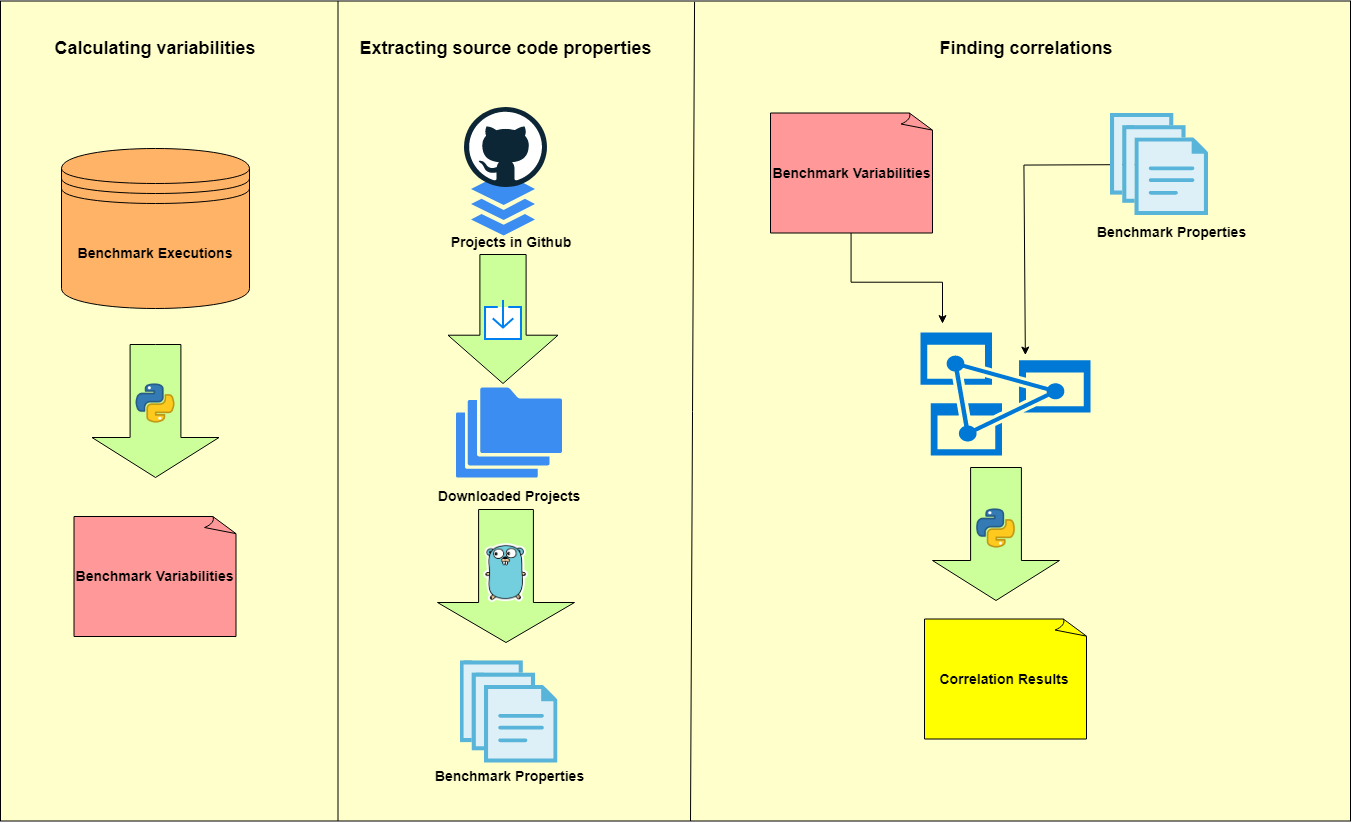
\includegraphics[width=\linewidth]{Methodology}
	\caption{3 main steps of the methodology.}
	\label{fig:Methodology}
\end{figure}

\section{Analyzing variabilities}
\label{Analyzing variabilities}

First part of this thesis involves doing a quantitative analysis by analyzing the given data set (This part refers to the 1. box in Figure \ref{fig:Methodology}). From this data set, I firstly extract the valid projects, i. e. choose the projects that have a positive number of individual benchmark results. Secondly, I calculate CV, RCIW95 and RCIW99 for each of benchmarks found in the dataset. For RCIW95 and RCIW99, I use a helper tool, called "pa tool" \cite{patool}, which helps me use the bootstrapping technique with randomly sampling, described in Section \ref{Microbenchmark variability}. The outcome of this part is explained in detail in Section \ref{Variabilities of benchmarks}.

\subsection{Dataset}

The dataset to analyze the variations from was given me from my supervisor Christoph Laaber. This dataset with a size of 43.8 MB contains \textbf{go-results.csv}, \textbf{go-results-2.csv} and 4 folders \textbf{cumulus-1 to cumulus-4}. In the \textbf{go-results-2.csv}, I find which project's result is on which relative path (which are in cumulus folders) and has how many individual results. \textbf{go-results.csv} differs from this file in having no commit of the projects. That's why, I start by analyzing \textbf{go-results-2.csv} in particular. In this file, I look for the column named "c1\_results": if the value in this column is above 0 (i.e., it is not -1), it means that there are results for that specific project on the special commit, which is found in the column "c1\_commit". From a total of 481 entries in this file, I get 230 projects which have individual results and filter them out. In the next step, I map the relative filepath of the project's result file to the name and commit of the project by querying the \textbf{go-projects.csv} file, which is to be found in every cumulus folder. In the end, I have all the valid projects with their results file.\\
\\
Results file of a projects looks like in Figure \ref{fig:exampleresults}. In this file, the middle part in the first column specifies the number of run, the second column specifies the benchmark including the relative path and file where the benchmark is located in, the forth column reports the execution time in nanoseconds, the fifth and sixth column are related to memory performance, bytes/operation and allocations/operation respectively.
 
\begin{figure}[H]
	\centering
	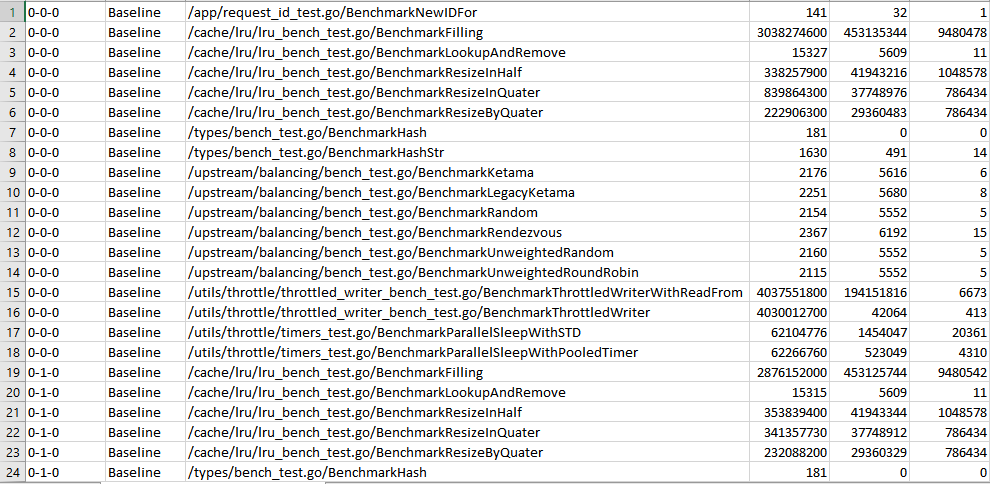
\includegraphics[width=\linewidth]{exampleresults}
	\caption{Example results file from \cite{ironsmile/nedomi}.}
	\label{fig:exampleresults}
\end{figure}
 
\subsection{Metrics as the variability indicators}

As described in Section \ref{Microbenchmark variability}, I orient myself at 3 main metrics to calculate the variabilities of the benchmarks. These are CV, RCIW95 and RCIW99 respectively. In this thesis, I'm only interested in the execution times, hence, I only take the forth column of the results file for each benchmark into consideration. To calculate the CV, I firstly find the standard deviation and mean of the execution times of each benchmark. Dividing the standard deviation by the mean gives me the CV. For the mathematical representation of CV, if the collection of benchmark results is called \textit{M}, then the CV of M can be shown as:
\[ cv(M) = \sigma _{M} / \mu _{M} \]
where $\sigma _{M}$ is the standard deviation and $\mu _{M}$ is the mean of the collection.\\
\\
For the RCIW part, I use a tool by Christoph Laaber, called "pa-tool" \cite{patool}. This tool works in the following way: For a given benchmark with all its execution times, it randomly samples a subset of the execution times and saves the mean of this new subset. This process is repeated for a considerable amount of time, e.g., 10000 times (number of bootstrap simulations), and returns the normally distributed set of mean execution times. This is because the distribution of the bootstrap means is normal due to the central limit theorem. Having the normal distribution is a requirement to take the confidence interval of the set. The tool finally gives a confidence interval of the new collection of means with a default significance level of 0.05. Listing \ref{lst:patool} illustrates an example output of pa-tool, showing the confidence interval of each benchmark in project ironsmile/nedomi after bootstrapping 10000 times with the 0.01 significance level \cite{ironsmile/nedomi}.
\begin{minipage}{\linewidth}

\begin{lstlisting}[caption=Example pa-tool results of \cite{ironsmile/nedomi}., label={lst:patool}, frame=single, breaklines=true, basicstyle=\small]
C:\Users\Mikael\pa>pa -bs 10000 -sig 0.01
"C:\Users\Mikael\go-calculation\pa_input_projects\1&ironsmile&nedomi_benchmarks.csv"
#Execute CIs:
# cmd = CI
# number of cores = 8
# bootstrap simulations = 10000
# significance level = 0.01
# statistic = Mean
# invocation sampling = Mean
# files 1 = [C:\Users\Mikael\go-calculation\pa_input_projects\1&ironsmile&nedomi_benchmarks.csv]
# files 2 = []

/app/request_id_test.go/BenchmarkNewIDFor;;;1.372879e+02;1.396515e+02;0.99
/cache/lru/lru_bench_test.go/BenchmarkFilling;;;2.950686e+09;2.982955e+09;0.99
/cache/lru/lru_bench_test.go/BenchmarkLookupAndRemove;;;1.527660e+04;1.532752e+04;0.99
/cache/lru/lru_bench_test.go/BenchmarkResizeByQuater;;;2.239956e+08;2.292164e+08;0.99
/cache/lru/lru_bench_test.go/BenchmarkResizeInHalf;;;3.551978e+08;4.518111e+08;0.99
/cache/lru/lru_bench_test.go/BenchmarkResizeInQuater;;;3.811996e+08;5.008146e+08;0.99
/types/bench_test.go/BenchmarkHash;;;1.813582e+02;1.834179e+02;0.99
/types/bench_test.go/BenchmarkHashStr;;;1.634015e+03;1.637060e+03;0.99
/upstream/balancing/bench_test.go/BenchmarkKetama;;;2.185776e+03;2.194403e+03;0.99
/upstream/balancing/bench_test.go/BenchmarkLegacyKetama;;;2.233333e+03;2.242545e+03;0.99
/upstream/balancing/bench_test.go/BenchmarkRandom;;;2.160121e+03;2.165439e+03;0.99
/upstream/balancing/bench_test.go/BenchmarkRendezvous;;;2.340515e+03;2.347833e+03;0.99
/upstream/balancing/bench_test.go/BenchmarkUnweightedRandom;;;2.157939e+03;2.164152e+03;0.99
/upstream/balancing/bench_test.go/BenchmarkUnweightedRoundRobin;;;2.123652e+03;2.130727e+03;0.99
/utils/throttle/throttled_writer_bench_test.go/BenchmarkThrottledWriter;;;4.030817e+09;4.036552e+09;0.99
/utils/throttle/throttled_writer_bench_test.go/BenchmarkThrottledWriterWithReadFrom;;;4.038926e+09;4.040731e+09;0.99
/utils/throttle/timers_test.go/BenchmarkParallelSleepWithPooledTimer;;;6.253588e+07;6.261951e+07;0.99
/utils/throttle/timers_test.go/BenchmarkParallelSleepWithSTD;;;6.182706e+07;6.191619e+07;0.99
#Total execution took 1.1923061s
	
\end{lstlisting}
\end{minipage}


\subsection{Benchmark Variabilities}
\label{Benchmark Variabilities}

Pa-tool requires the benchmarks of a project to be sorted in alphabetical order, along with its number of run and the execution time. After I have all the valid projects with their results file, I firstly create input CSV files for the pa-tool to function accordingly. In the next step, I iterate through input files for pa-tool and run the pa-tool for each project 2 times, once with the significance level of 0.05 and once with 0.01, both having 10000 bootstrap simulations. From the boundaries of the confidence interval acquired from the pa-tool, I calculate RCIW values by substracting the left boundary from the right boundary, divided by the mean of the benchmark results. For the mathematical representation, if we call the benchmark \textit{B}, collection of benchmark results \textit{M}, the normal distributed output of pa-tool $M_{n}$, and the confidence interval of $M_{n}$ \textit{CI}, then the RCIW value of a benchmark can be shown as:
\[ RCIW(B) = ({CI_{R}} - {CI_{L}}) / \mu _{M} \]
where $CI_{R}$ is the right, $CI_{L}$ is the left boundary of the confidence interval and $\mu _{M}$ is the mean of benchmark's execution results.

\noindent As a result of this calculation, I get RCIW95 for the results with 0.05 significance level of confidence interval, and RCIW99 for the results with 0.01 significance level of confidence interval. For the CV part of each benchmark, I use \textit{mean()} and \textit{stddev()} from Python's \textit{statistics} module\cite{pythonsta}.\\
\\
Within the end of calculating CV, RCIW95 and RCIW99 of each benchmark, I write all the benchmarks into the \textbf{benchmark\_variabilities.csv} file, which shows the name of the project, the specific benchmark, number of executions, and mean, CV, RCIW95 and RCIW99 of the benchmark respectively. Listing \ref{fig:finalcsv} shows the first lines of \textbf{benchmark\_variabilities.csv}.

\begin{figure}[H]
	\centering
	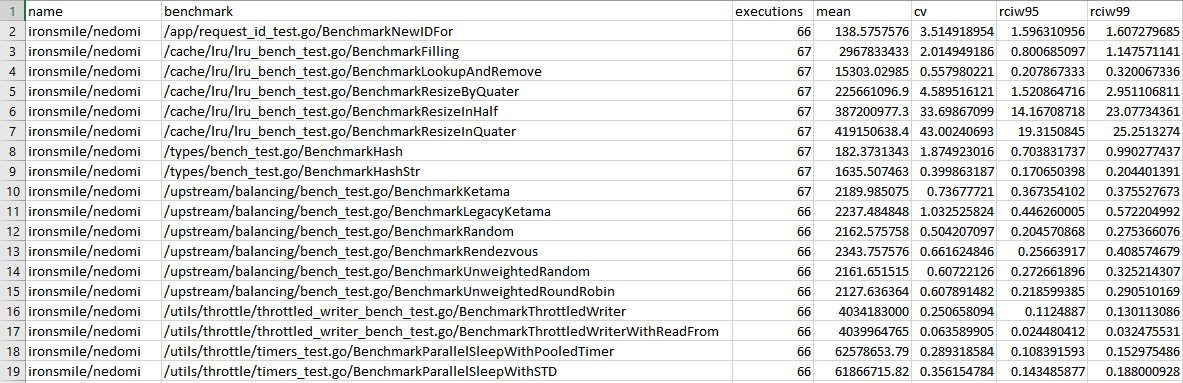
\includegraphics[width=\linewidth]{finalcsvexample}
	\caption{First lines from the benchmark\_variabilities.csv file involving variability values for \cite{ironsmile/nedomi}.}
	\label{fig:finalcsv}
\end{figure}

\section{Extracting source code features}

This is the second part of the study, which involves extracting the source code properties of benchmarks, for which I calculated the variabilities in Section \ref{Analyzing variabilities}. This part consists of a downloading projects from Github, extracting information about all kinds of functions (normal, test and benchmarks) in these projects and finally creating CSV files for each project, having the benchmarks and their properties, which can visually be seen in the second box of Figure \ref{fig:Methodology}. Results of this part are to be found in Section \ref{Extracted source code features}.

\subsection{Decision on source code properties}

Prior to programming for each of the parts, I do a qualitative analysis to decide on the properties that I want to extract for each benchmark. For this, I start by analyzing some of the benchmarks with particularly high variabilities and look for the properties that come up in these. While this gives me some basic ideas about what to analyze, I also scroll through the standard library of Go \cite{gopackages} and look for the libraries, which in my opinion might make an impact to the variability of the benchmarks. At the time of doing that, my particular inspectation goes to the libraries which implement functionalities about handling file IO, http calls and other functionalities that might otherwise make an impact on the variability.\\
\\
As a second source for the source code properties, I have a look at the Go Programming Language \cite{go} and its language properties. Near features such as data structures, control flow elements and error handling mechanisms, Go is also full equipped with concurrency related features, which enable developers to code parallel programs without having to code for underlying data structures in first place. With this, I put language related features on top of usage of standard libraries whilst deciding for the source code properties. Additionally, I look up for source code metrics that are often used/extracted in the literature and find cyclomatic complexity as a metric to measure the depth of control flow graph of a function \cite{shepperd1988critique}.\\
\\
Finally, I create the list of properties in Table \ref{table:sourcecodeprop} to analyze when extracting information out of functions. In total, there are 4 different types of properties that I analyze. First one is the usage of specified standard library. In this type, there are 31 libraries that can play a role on the variability of the benchmarks. In particular, I inspect \textbf{io, io/ioutil} which represents file I/O operations; \textbf{net/http, net/http/httptest, net/http/httptrace, net/http/httputil} which represent http calls and other http related functions. All the remaining properties are for me of interest as well: For instance, I wonder if the usage of random functions has an impact on the variability and look for the occurences of \textbf{math/rand}; similarly, I'm interested in the usage of synchronization primitives and seek for \textbf{sync, sync/atomic} to see whether count of usage of this library within a benchmark affects the benchmark in a significant way. Second property type in the list is signature of the function, which stands for the properties that are directly related with the function. In this type there are 6 properties, which can be extracted by looking at the place of function's definition and the identifiers of the function. Third property type is called body of the function, which contains all the properties that can be extracted from the body of the benchmarks. For the variability of the benhcmark, these can also be a predictor of stability. Last property type is other, which has cyclomatic complexity.\\
\\
For the extraction of these properties, I use the methodology of parsing the Abstract Syntax Tree of a source code file. While signature properties require only the inspection of function declarations within the AST, the other 3 types require analysis of the body of the function within the declaration, going into a deeper level.

\begin{table}[H]
	\caption{List of source code properties.}
	\label{table:sourcecodeprop}
	\resizebox{\textwidth}{!}{%
		\begin{tabular}{@{}llr@{}}
			\toprule
			\textbf{Property Type} & \textbf{Property Name} & \textbf{Explanation} \\ \midrule
			\multirow{31}{*}{Standard library usage} & bufio & Library to handle buffer actions. \\
			& bytes & Library to manipulate byte slices. \\
			& crypto & Library that has common cryptographic constants. \\
			& database/sql & Library for database interactions. \\
			& encoding & \multirow{5}{*}{Libraries for handling different type of encodings.} \\
			& encoding/binary &  \\
			& encoding/csv &  \\
			& encoding/json &  \\
			& encoding/xml &  \\
			& io & \multirow{2}{*}{Libraries that hold io primitives and io functionalities.} \\
			& io/ioutil &  \\
			& math & \multirow{2}{*}{Libraries for math functions and random implementations.} \\
			& math/rand &  \\
			& mime & Library implementing parts of MIME spec. \\
			& net & Library for handling network I/O. \\
			& net/http & \multirow{4}{*}{\begin{tabular}[c]{@{}c@{}}Libraries implementing HTTP client and server, \\ utilities for HTTP testing, mechanisms to trace events \\ and other HTTP utility functions.\end{tabular}} \\
			& net/http/httptest &  \\
			& net/http/httptrace &  \\
			& net/http/httputil &  \\
			& net/rpc & \multirow{2}{*}{Libraries that implement remote procedure calls for objects.} \\
			& net/rpc/jsonrpc &  \\
			& net/smtp & Library to handle Simple Mail Transfer Protocol. \\
			& net/textproto & \begin{tabular}[c]{@{}c@{}}Library that implements generic support for \\ text based request/response protocols.\end{tabular} \\
			& os & Library to handle OS functionality. \\
			& os/exec & Library to run external commands. \\
			& os/signal & Library to access incoming signals. \\
			& sort & Library to sort slices and user defined collections. \\
			& strconv & \begin{tabular}[c]{@{}c@{}}Library that implements conversion to and from \\ string representations.\end{tabular} \\
			& sync & \multirow{2}{*}{\begin{tabular}[c]{@{}c@{}}Libraries that implement basic synchronization primitives \\ and low-level atomic memory primitives.\end{tabular}} \\
			& sync/atomic &  \\
			& syscall & \begin{tabular}[c]{@{}c@{}}Library that implements an interface to \\ low-level operating system primitives.\end{tabular} \\
			\midrule
			\multirow{6}{*}{Signature of the function} & pkgfiles & Files in the package where the function belongs to. \\
			& fileloc & Lines of code of the file where the function belongs to. \\
			& namelength & Length of the name of the function. \\
			& parameters & Parameters of the function. \\
			& returns & Return values of the function. \\
			& loc & Lines of code of the function. \\
			\midrule
			\pagebreak
			\multirow{21}{*}{Body of the function} & funccalls & Function calls within the function. \\
			& loops & For and while loops within the function. \\
			& nestedloops & Nested for/while loops within the function. \\
			& channels & Channel creations within the function. \\
			& sends & Sending data to the channel within the function. \\
			& receives & Receiving data from the channel within the function. \\
			& closes & Channel terminations within the function. \\
			& gos & Go keywords (new threads) within the function. \\
			& concrranges & Channel loops within the function. \\
			& selects & Select statements within the function. \\
			& selectcases & Cases in select statements within the function. \\
			& variables & \multirow{4}{*}{\begin{tabular}[c]{@{}c@{}}Variable, pointer, slice and map declarations \\ within the function.\end{tabular}} \\
			& pointers &  \\
			& slices &  \\
			& maps &  \\
			& ifelses & If-else statements within the function. \\
			& switches & Switch statements within the function. \\
			& switchcases & Cases in switch statements within the function. \\
			& panics & Panic statements within the function. \\
			& recovers & Recover statements within the function. \\
			& defers & Defer statements within the function. \\
			\midrule
			Other & cyclomaticcomplexity & Cyclomatic complexity of the function. \\
		\end{tabular}%
	}
\end{table}



\subsection{Downloading projects}

To download all the valid projects that resulted with 4589 benchmarks in the first analysis, I firstly create a little CSV file which stores the name of the projects and its commit, where the execution results are from. I then write a Python script, which reads this file and downlods the projects sequentially from Github. For downloading, I use Go's \textit{get CLI flag}, as this is intended to download and install a Go project along with its dependencies. However, downloading these projects with:
\begin{lstlisting}
	go get github.com/{owner_name}/{project_name}
\end{lstlisting}

\noindent does not suffice, because the commits of these projects are from a time when Go Modules did not used to exist. This means, at the time of these commits projects had their own package management tools, which ensured getting the right dependencies for the project \cite{packagemanagement}. Because projects had their own GOPATH environment back then, I create a GOPATH for each of the projects prior to downloading them. On one hand, I ensure that their dependencies from their commits can be stored in their own GOPATH, on the other hand, I avoid clashing dependencies from other projects, which would then share the same GOPATH for all the dependencies. Post download, I then use a locally installed Git to checkout the project folder from master to the given commit in the CSV file. As an output, I get a CSV file containing name, commit and installed path of each project. This output file is useful for the parser tool that can iterate through different projects, which is explained in the next section. Figure \ref{fig:downloadproject} illustrates the process of downloading projects.

\begin{figure}[H]
	\centering
	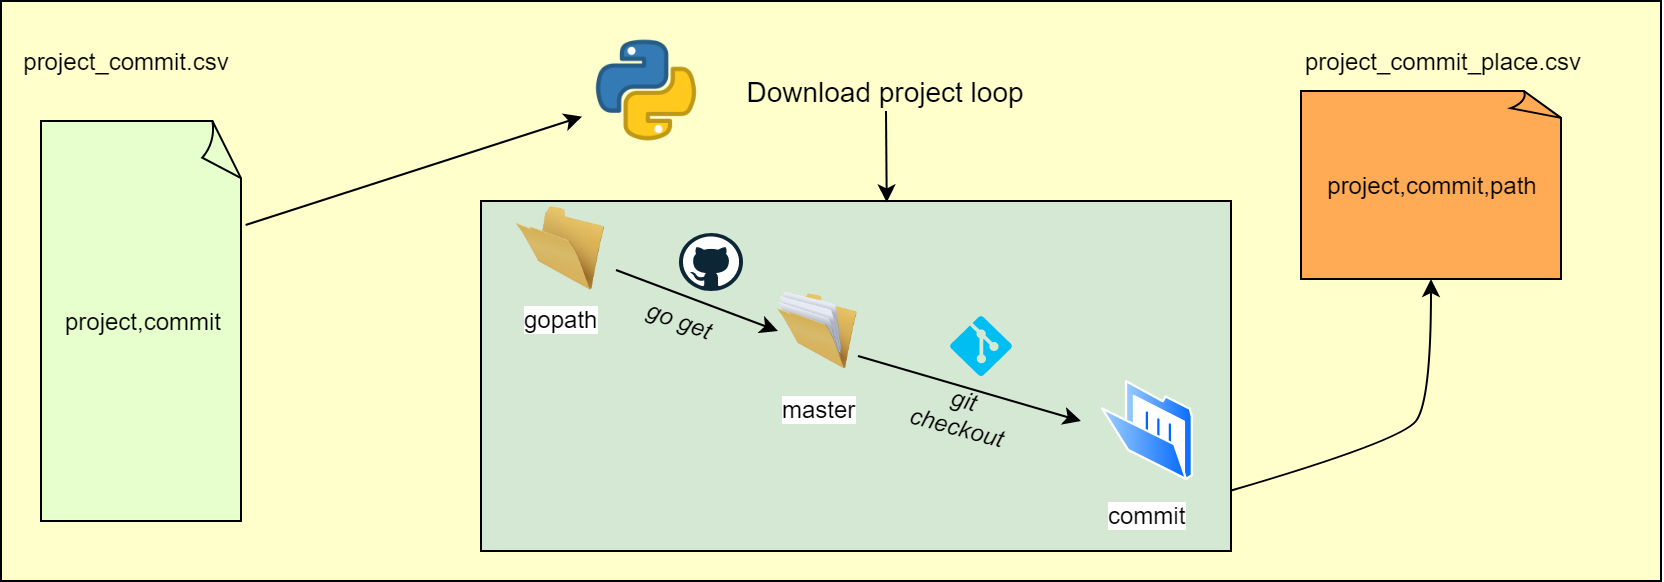
\includegraphics[width=\linewidth]{downloadproject}
	\caption{Process of downloading projects from Github.}
	\label{fig:downloadproject}
\end{figure}


\noindent Extracting source code properties in this thesis consists of two main parts. First part has to do with AST parsing of source code files to extract all the functions within a project. Second part is about using a callgraph CLI tool which resides in Go's \textit{golang.org/x/tools/cmd/} repository\cite{callgraphtool}. In particular, I use the parser tool in the first part to create a CSV file from a project which has all the functions with their source code features. Following that, I use the callgraph tool to iterate through the callgraph of each benchmark found in the resulting CSV file from the parser tool in order to find all the called functions from a benchmark. This way, I'm able to match all the called functions from the benchmark in the first CSV file and calculate the sum of each feature value for the benchmark. Output of the callgraph tool is a CSV file for the project, which contains only the benchmark functions with their source code properties.\\
\\
For both of the parts I use Go programming language as it offers great functionabilities when it comes to parsing Go's source code files and collect source code information. I present the resulting tools "Prophunt" and "Callgraph Analyzer" in the next sections.

\subsection{Prophunt}
\label{Prophunt}
After having all the projects residing in their own GOPATHs, next step is to start with parsing the source code of each file found in a project. But before that, there is still a step that needs to be taken, which is getting the dependencies. Downloading the projects with "go get" without any further flag only causes downloading and installing them in the specified GOPATH, fetching only the dependencies that can be fetched via Go Modules and only for the master commit. However, to be able to parse the source code correctly and have no compilation errors, all the dependencies that are required for that special commit need to be fetched. Because of that reason, I firstly implement a mechanism to iterate through all the project paths, set the GOPATH accordingly, call \textit{"go get -t ./..."} inside the project's root folder and use \textit{deps/fetch.go/Fetch} method from Christoph Laaber's GoABS implementation \cite{sealuzh/goabs}.

\begin{figure}[H]
	\centering
	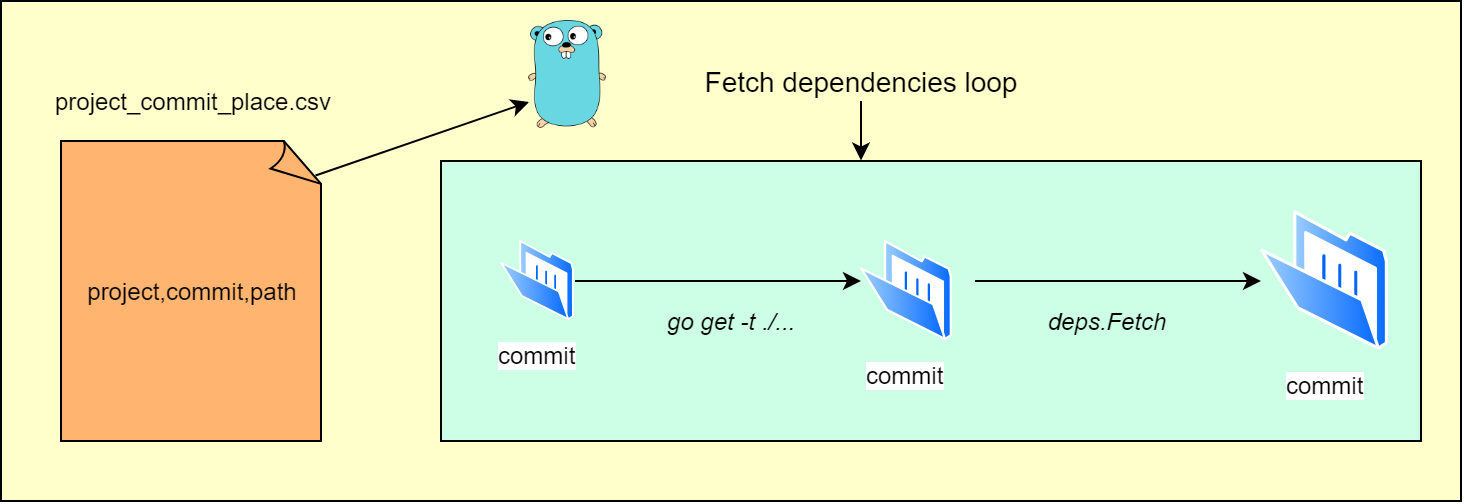
\includegraphics[width=\linewidth]{fetchdeps}
	\caption{Process of fetching dependencies for each project.}
	\label{fig:fetchdeps}
\end{figure}

\noindent Figure \ref{fig:fetchdeps} shows how this process runs in Go. The optional "-t" flag of \textit{go get} ensures the installation of all required test packages and the latter \textit{./...} tells \textit{go get} to fetch all dependencies for this project. This command is crucial, since without getting dependencies for test packages some of the source code files cannot be compiled correctly, which leads to not being able to parse them correctly, using Prophunt. For all the projects with their specific commits, which are compabible with Go Modules, this step suffices in terms of being ready to be parsed. However, there are projects which use other package management tools \cite{packagemanagement}. For these kind of projects, I use \textit{deps.Fetch} method and give it the path of the project, from which it automatically extracts GOPATH of the projects and uses one of the preinstalled dependency management tools to get the dependencies. As of writing this thesis, this method has support for the tools (which need to be installed before using the method) listed in Table \ref{dependencymanagementtools}.

\begin{table}[H]
\caption{List of dependency management tools supported in GoABS}
\label{dependencymanagementtools}
\begin{longtable}[c]{@{}ll@{}}
	\toprule
	Tool & Repo \\* \midrule
	\endfirsthead
	%
	\endhead
	%
	\bottomrule
	\endfoot
	%
	\endlastfoot
	%
	Get & built-in \\
	dep & https://github.com/golang/dep \\
	Glide & https://github.com/Masterminds/glide \\
	Godep & https://github.com/tools/godep \\
	Govendor & https://github.com/kardianos/govendor \\
	gvt & https://github.com/FiloSottile/gvt \\
	govend & https://github.com/govend/govend \\
	trash & https://github.com/rancher/trash \\
	gom & https://github.com/mattn/gom \\
	gopm & https://github.com/gpmgo/gopm \\
	Gogradle & https://github.com/blindpirate/gogradle \\
	gpm & https://github.com/pote/gpm \\
	glock & https://github.com/robfig/glock \\* \bottomrule
\end{longtable}
\end{table}


\noindent I install these tools prior to fetching dependencies in my Ubuntu 18.04 Virtual Machine (VM) environment. After fetching dependencies for all the projects, I am ready for the next step in Prophunt, which is parsing.

\paragraph{Parsing}

I firstly start my parsing processes by importing Go's \textbf{parser} library, and giving its \textit{ParseFile} method some source code files written in Go and the \textit{parser.ParseComments} mode as parameters to parse everything including comments in a file. This method, unless errors occure, returns an \textbf{*ast.File} instance, which represents a file in Go environment. This instance, as shown in Listing \ref{astFile}, has all the information about a .go file. This return value can now be investigated by using its attributes, for example, \textit{*ast.File.Name} gives name of the package this .go file belongs to.

\begin{lstlisting}[caption=*ast.File declaration in Go., label={astFile}, language=Go, frame=single]
	type File struct {
	Doc        *CommentGroup   // associated documentation; or nil
	Package    token.Pos       // position of "package" keyword
	Name       *Ident          // package name
	Decls      []Decl          // top-level declarations; or nil
	Scope      *Scope          // package scope (this file only)
	Imports    []*ImportSpec   // imports in this file
	Unresolved []*Ident        // unresolved identifiers in this file
	Comments   []*CommentGroup // list of all comments in the source file
	}
\end{lstlisting}

\noindent Since I am interested in the function declarations in the file, I investigate the \textbf{Decls} slice and search for the function declarations in this slice. A function declaration is defined as \textbf{*ast.FuncDecl} within this library, and has attributes such as \textbf{Doc}, \textbf{Recv}, \textbf{Name}, \textbf{Type} and \textbf{Body}, as in Listing \ref{funcdecl}. From the \textbf{Type} attribute, one can read information about parameters and return values of the function. From the \textbf{Recv} attribute, the receiver of the method can be read. Rest of the properties that I look for are located in the \textbf{Body} of the function.


\begin{lstlisting}[caption=*ast.FuncDecl declaration in Go., label={funcdecl}, language=Go, frame=single]
FuncDecl struct {
	Doc  *CommentGroup // associated documentation; or nil
	Recv *FieldList    // receiver (methods); or nil (functions)
	Name *Ident        // function/method name
	Type *FuncType     // function signature: parameters, results, 
					   // and position of "func" keyword
	Body *BlockStmt    // function body; or nil for external (non-Go) function
}
\end{lstlisting}

\noindent Signature properties are trivially extracted from the \textbf{*ast.FuncDecl}, however, for all the body, standard library usage and other type of properties, one needs to know what to look for inside the \textbf{Body} of the \textbf{*ast.FuncDecl}. To this end, I firstly look for Go's "A Tour of Go" documentation \cite{atourofgo} and find code examples about properties of the language. While one can use these code examples in the programming environment, I aim for a GUI approach to better understand how to look for properties in the bodies of functions. Fortunately, I come across a web application from yuroyoro \cite{goastviewer}, which offers a GUI to visualize a Go AST, given Go source code. Listing \ref{yuroyoro} shows an example output from the AST Viewer of a main function with a "Hello Golang" print on the stdout.

\begin{minipage}{\linewidth}
\begin{lstlisting}[caption=Sample output from yuroyoro's Ast Viewer \cite{goastviewer}., label={yuroyoro}, language=Go, frame=single, ]
	23  .  .  1: *ast.FuncDecl {
	24  .  .  .  Name: *ast.Ident {
	25  .  .  .  .  NamePos: 7:6
	26  .  .  .  .  Name: "main"
	27  .  .  .  .  Obj: *ast.Object {
	28  .  .  .  .  .  Kind: func
	29  .  .  .  .  .  Name: "main"
	30  .  .  .  .  .  Decl: *(obj @ 23)
	31  .  .  .  .  }
	32  .  .  .  }
	33  .  .  .  Type: *ast.FuncType {
	34  .  .  .  .  Func: 7:1
	35  .  .  .  .  Params: *ast.FieldList {
	36  .  .  .  .  .  Opening: 7:10
	37  .  .  .  .  .  Closing: 7:11
	38  .  .  .  .  }
	39  .  .  .  }
	40  .  .  .  Body: *ast.BlockStmt {
	41  .  .  .  .  Lbrace: 7:13
	42  .  .  .  .  List: []ast.Stmt (len = 1) {
	43  .  .  .  .  .  0: *ast.ExprStmt {
	44  .  .  .  .  .  .  X: *ast.CallExpr {
	45  .  .  .  .  .  .  .  Fun: *ast.SelectorExpr {
	46  .  .  .  .  .  .  .  .  X: *ast.Ident {
	47  .  .  .  .  .  .  .  .  .  NamePos: 8:2
	48  .  .  .  .  .  .  .  .  .  Name: "fmt"
	49  .  .  .  .  .  .  .  .  }
	50  .  .  .  .  .  .  .  .  Sel: *ast.Ident {
	51  .  .  .  .  .  .  .  .  .  NamePos: 8:6
	52  .  .  .  .  .  .  .  .  .  Name: "Printf"
	53  .  .  .  .  .  .  .  .  }
	54  .  .  .  .  .  .  .  }
	55  .  .  .  .  .  .  .  Lparen: 8:12
	56  .  .  .  .  .  .  .  Args: []ast.Expr (len = 1) {
	57  .  .  .  .  .  .  .  .  0: *ast.BasicLit {
	58  .  .  .  .  .  .  .  .  .  ValuePos: 8:13
	59  .  .  .  .  .  .  .  .  .  Kind: STRING
	60  .  .  .  .  .  .  .  .  .  Value: "\"Hello, Golang\\n\""
	61  .  .  .  .  .  .  .  .  }
	62  .  .  .  .  .  .  .  }
	63  .  .  .  .  .  .  .  Ellipsis: -
	64  .  .  .  .  .  .  .  Rparen: 8:30
	65  .  .  .  .  .  .  }
	66  .  .  .  .  .  }
	67  .  .  .  .  }
	68  .  .  .  .  Rbrace: 9:1
	69  .  .  .  }
	70  .  .  }
\end{lstlisting}
\end{minipage}

\noindent Generally, the properties to collect are reachable from the \textbf{Body} by querying for the correct parser instance. Table \ref{table:propsast} presents how I extract these properties or which data structure I aim for when visiting the nodes in a function declaration. For the cyclomatic complexity, I adapt the calculation to an existing calculation approach by fzipp/gocyclo \cite{gocyclo}. 

\begin{table}[H]
\caption{Extraction of properties based on parser library.}
\label{table:propsast}
\begin{longtable}[c]{@{}ll@{}}
	\toprule
	\textbf{Property Name} & \textbf{According Parser Instance / Extraction Method} \\* \midrule
	\endfirsthead
	%
	\endhead
	%
	\bottomrule
	\endfoot
	%
	\endlastfoot
	%
	funccalls & *ast.CallExpr \\
	loops & *ast.ForStmt / *ast.RangeStmt \\
	nestedloops & none, counting loops inside loops \\
	channels & *ast.ChanType \\
	sends & *ast.SendStmt \\
	receives & *ast.UnaryExpr.Op being "\textless{}-" \\
	closes & *ast.CallExpr having name "close" \\
	gos & *ast.GoStmt \\
	concrranges & none, counting loops with channel ranges \\
	selects & *ast.SelectStmt \\
	selectcases & *ast.SelectStmt.Body.List length \\
	variables & \begin{tabular}[c]{@{}l@{}}*ast.DeclStmt --\textgreater *ast.GenDecl\\ or *ast.AssignStmt right side being *ast.BasicLit\end{tabular} \\
	pointers & \begin{tabular}[c]{@{}l@{}}*ast.AssignStmt right side having\\ *ast.UnaryExpr.Op being "\&"\end{tabular} \\
	slices & *ast.ArrayType \\
	maps & *ast.MapType \\
	ifelses & *ast.IfStmt \\
	switches & *ast.SwitchStmt \\
	switchcases & *ast.SwitchStmt.Body.List length \\
	panics & *ast.CallExpr having name "panic" \\
	recovers & *ast.CallExpr having name "recover" \\
	defers & *ast.DeferStmt \\
	cyclomaticcomplexity & \begin{tabular}[c]{@{}l@{}}calculated by counting each instance of:\\ *ast.FuncDecl\\ *ast.IfStmt\\ *ast.ForStmt\\ *ast.RangeStmt\\ *ast.CaseClause\\ *ast.CommClause\\ *ast.BinaryExpr\\ within the function\end{tabular} \\
	standard library usages & checking resolved funccalls within a function \\* \bottomrule
\end{longtable}
\end{table}

\noindent To be able to parse each function correctly and later match them with the output of the callgraph tool, I need to resolve the package of the function or the package of the receiver of the method if a receiver exists. Unfortunately, without having types info for the file to be parsed, this is impossible unless all the information is found in the same file. In practice, this is rarely the case.

\paragraph{Package packages}

I use a library called \textbf{packages} from Go's \textit{golang.org/x/tools/go/} repository  \cite{packages}, which offers the functionality to load a package's related info to the programming environment. This comes as a perfect solution to the problem of resolving types, since it gives all the found .go files in the folder with their according package and a slice of \textbf{*ast.File} for the files that compile within the folder. Furthermore, since it automatically parses all the files, there is no need to parse all the files one by one as I practiced in the previous section. The crucial feature of this functionality is, that it automatically generates a \textbf{*types.Info} instance for each package, which can later be used to query for the resolving type of an existing \textbf{*ast.Ident} node in the AST tree. Best practice to use this package is by giving the path of a folder containing Go source files as a parameter to the configuration of \textit{packages.Load}, while also telling the configuration to include all test files.\\
\\
Go's standard practice tells to put the test files in the "\_test" version of the package found in the folder. If that is the case for a folder, \textit{packages.Load} returns both the normal and "\_test" version of the package with their compiled .go files. However, in the dataset that I analyze there are projects which don't follow this practice, hence, they use only one package per folder and include the tests in the same package. In that case, \textit{packages.Load} returns all the .go files in the "package [package.test]" package.\\
\\
Having \textbf{packages} library as the skeleton to my parsing technique, I create \textbf{Prophunt}, which is a tool that takes a project folder as a parameter and starts walking all the folders of the project, starting from the root folder. For each folder, resulting packages are acquired via \textit{packages.Load} and function declarations are extracted for each of the compiling .go files. Then, the properties of each function is collected from the functions, using algorithms that aim for the according parser instance or extraction method of the property to be extracted. At the end of visiting all possible functions, the functions are written into a CSV file which includes all 3 kinds of functions from a project, namely: \textbf{normal}, \textbf{test} and \textbf{benchmark} functions. Figure \ref{fig:prophunt} illustrates the workflow of Prophunt. Simply explained, it takes the CSV from Python downloader script to iterate through projects, creates a map containing each function and their properties, and fills it by loading each package, filtering the functions and extracting their properties. At the end of visiting all folders of a project, the map is transformed into a CSV for the project, which is saved in \textit{Prophunt\_Output} folder. For convenience, also an \textit{index.csv} file is written in this folder for later usage with callgraph analyzer, which contains the names and Prophunt\_Output paths of the projects.

\begin{figure}[H]
	\centering
	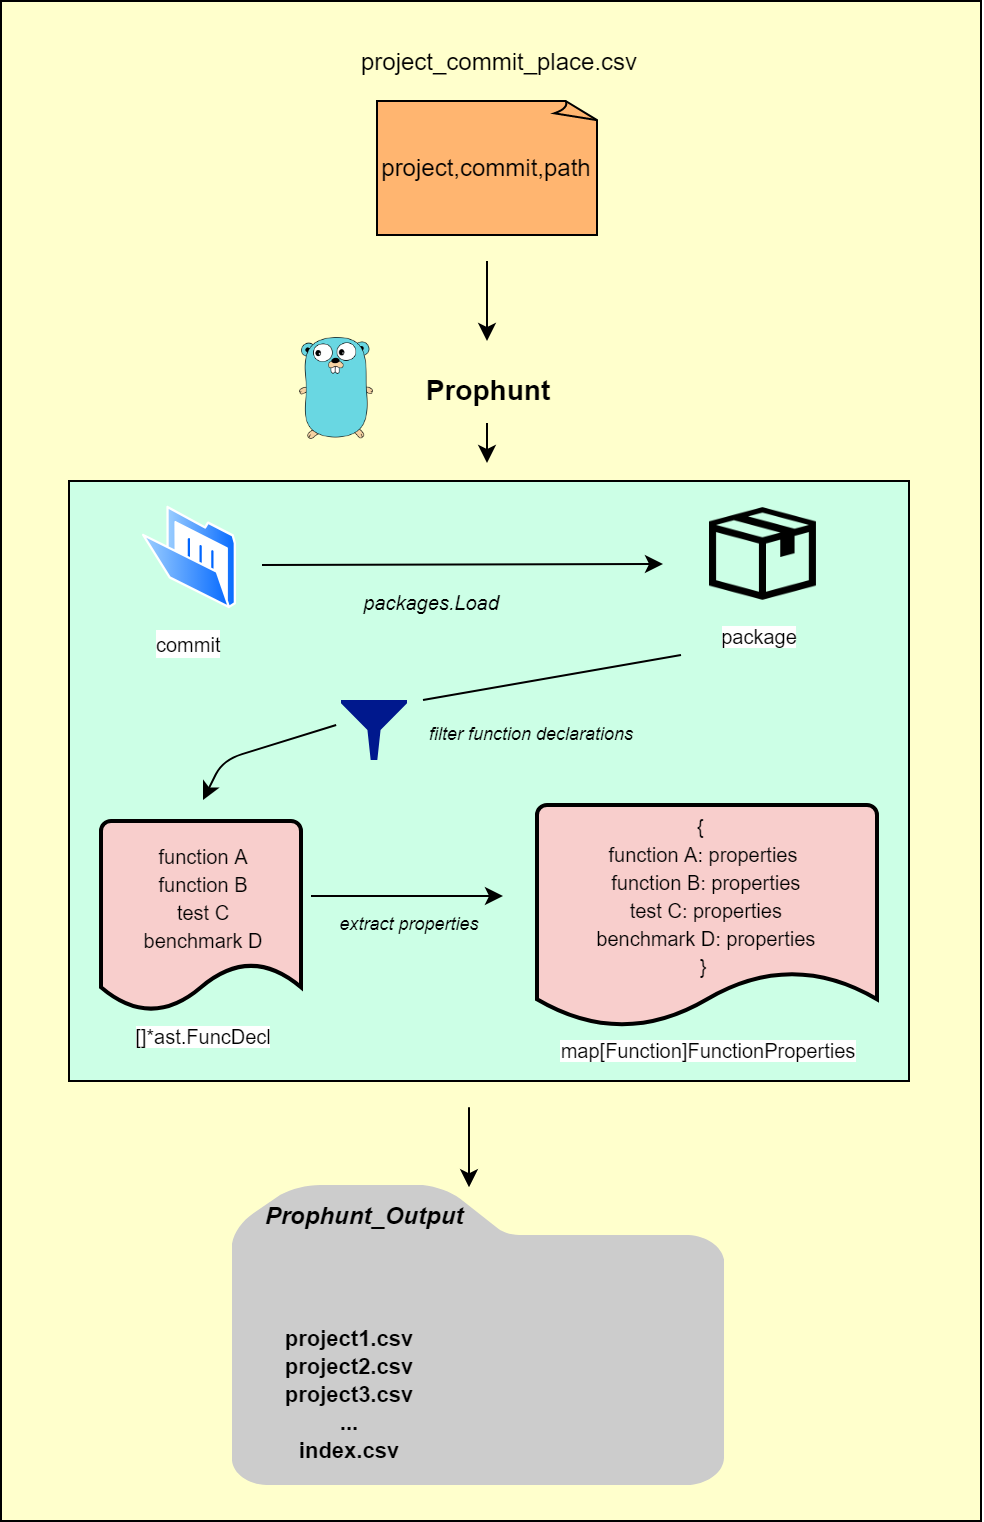
\includegraphics[width=\linewidth]{prophunt}
	\caption{Workwise of Prophunt iterating through downloaded projects.}
	\label{fig:prophunt}
\end{figure}


\subsection{Callgraph Analyzer}
\label{Callgraph Analyzer}

Creating Prophunt outputs for all the projects is only half of the story, because the information in these CSV files are only relevant to the functions themselves, i.e., having only Prophunt outputs I am limited to properties of an individual function. However, to make a proper correlation analysis, it is interesting and important to look at the callgraphs of the benchmarks, because these reveal information about all the functions that are called by a benchmark. The idea behind the callgraph analyzer is to build a directed graph, which has function nodes and edges between function nodes respresenting a function call. In such a graph, the outgoing node of an edge is the caller, and the incoming node of an edge is the callee. Having such a datastructure can be used to return all the visited functions from a benchmark. To this end, I search for a tool which can in some way return me the edges between functions, which in whole builds the callgraph of the project. Fortunately I come across the callgraph CLI tool, which resides in Go's \textit{golang.org/x/tools/cmd/} repository\cite{callgraphtool}.\\
\\
\paragraph{callgraph CLI tool} The tool expects several flags to give the callgraph of a project as output: the first and most important flag is the algorithm ("-algo") that is used to create the callgraph. Under 4 different algorithm options (\textbf{Static}, Class Hierarchy Analysis (\textbf{cha}), Rapid Type Analysis (\textbf{rta}) and inclusion-based Points-to Analysis (\textbf{pta})), I use inclusion-based Points-to Analysis. \textbf{pta} is often referred as Points-to-Analysis and is used in computer science as a static code analysis technique. In its pure form, the algorithm tries to find about which pointer or heap reference can be pointing to which variable or storage location at the runtime. This algorithm, as \textbf{rta}, requires a whole program to give correct output, and includes only functions that are reachable from main \cite{callgraphtool}. This means, that if a benchmark has function calls that are not included in the main or tests of the whole project, this benchmark will likely not be included in the callgraph tool's output, which is the only analyzed drawback by me. The other flags of the tool include "-test", which is to enable creating callgraphs of tests as well and "-format", which is to format the output of the callgraph tool. Using "-format" with "digraph" gives all the edges in form:

\begin{lstlisting}[caption=Output format of callgraph CLI tool., label={callgraphcli}, language=Go, frame=single] 
"package.functionA" "package.functionB"
"(package.receiver).functionC" "(*package.receiver).functionD"
"(package.receiver).functionE" "(package.receiver).functionC"
\end{lstlisting}

\noindent where each \textbf{functionX} is defined by the signature of the function in a specific way. For instance, if a function is a method, it has the resolved package of the receiver concatenated with the receiver in parantheses before the function name. If the receiver is a pointer type, it has an asterisk at the beginning of the receiver's resolved package. In any other case, the function has the resolved package followed by the function name. Listing \ref{callgraphcli} shows all kinds of examples explained here.\\
\\
Next step in order to have a sound directed graph of a project is to find a datastructure, which can store all the nodes with their edges. For this, I import the graph library of \textbf{gonum/gonum} \cite{gonum/gonum}, which is a performant library that has implementations of different graph types. In particular, I use the \textbf{*simple.DirectedGraph} data structure to feed all the edges that can be acquired from the project. Once this graph is fully fed with every found edge from the callgraph tool, the graph can be queried for all the callees of a benchmark.

\begin{figure}[H]
	\centering
	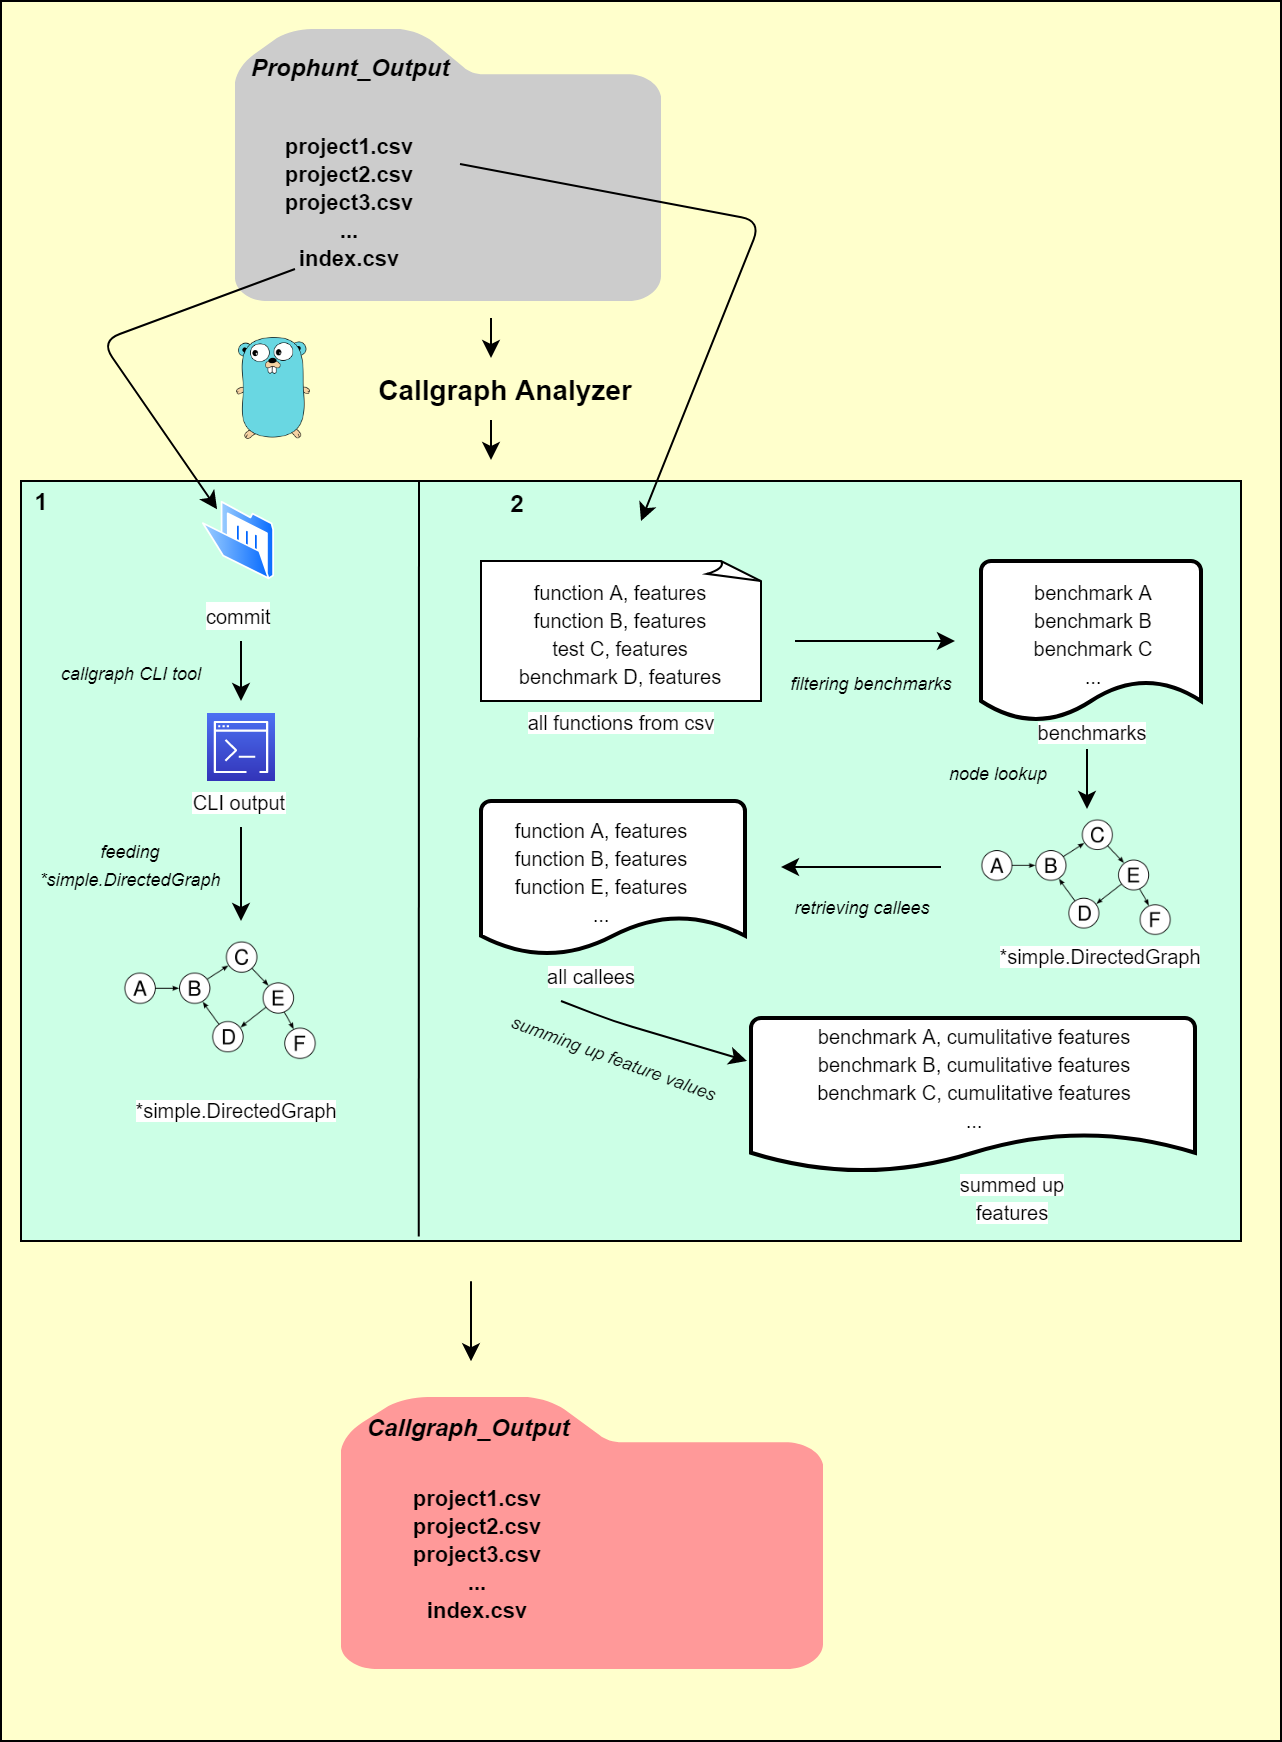
\includegraphics[width=\linewidth]{callgraph}
	\caption{Workwise of Callgraph Analyzer iteration through all parsed projects.}
	\label{fig:callgraph}
\end{figure}
 
\noindent Figure \ref{fig:callgraph} shows how Callgraph Analyzer works. Similar to Prophunt, Callgraph Analyzer takes the full path of the project to be analyzed from Prophunt\_Output's index.csv. A single loop execution consists of 2 phases. In the first phase, the callgraph tool is called for each of the projects folder because of 2 reasons: (1) a project might not have a main in the root folder, hence, the callgraph fails to create the edges and (2) there might exist more than 1 main in the whole project structure and they may have different scopes for the functions across the project. After each call of the CLI tool, the output is read and the nodes and their edges are collected. These are directly fed to the \textbf{*simple.DirectedGraph} instance of the project. Due to the precautions in the implementation of \textbf{*simple.DirectedGraph}, a node cannot be added to the graph twice, hence, I eliminate edges that occured in a previous output from the process and only feed the nodes if they were not in the graph before. A full walk through the project path results as a full callgraph of a project.\\
\\
In the second phase of the same loop execution, according CSV file for the project is read from Prophunt\_Output folder and its benchmarks are filtered. Having all benchmarks on one place, a lookup for all direct callees of one benchmark node can be made by using \textit{simple.From()} method, when the node of the benchmark is given as a parameter. Since I am interested in not only the direct callees but also all reachable nodes from a benchmark node, I implement a recursive algorithm which calls \textit{simple.From()} method for all the nodes that can be visited from the initial benchmark node. This ensures collecting all the reachable nodes in the callgraph, and as a next step I search for the callees in the according projectX.csv file. If reachable nodes are present in the .csv file of the project, I collect their .csv entries to later sum up all the property values, resulting into the benchmark's cumulitative properties. Note that namelength and parameters are not summed up, as their cumulitative value is not useful for the correlation analysis. Using this methodology, there is 3 possible outcomes for every benchmark analzed by Prophunt: (1) the benchmark cannot be found in the callgraph, resulting into a nil node in the programming environment. In this case, I skip this benchmark and do not record it in the output; (2) the benchmark is found in the callgraph, however, there is no reachable node from this benchmark, either because there was a compilation error in the callgraph CLI tool, or the callees of the benchmark were not reachable from main of the project; (3) the benchmark is found in the callgraph and there is at least 1 reachable node from the benchmark in the callgraph. For the completeness of the results, I anticipate that there are not many occurences of the first and second outcomes, nevertheless, the numbers are reported in the \ref{Extracted source code features} Section. Finally, Callgraph Analyzer gives an output folder called Callgraph\_Output with a CSV for each project containing only the benchmarks with their cumulitative property values, as well as an index.csv file which is used later at the correlation analysis.

\section{Finding correlations}

Third and last part of the study is to find correlations between source code features of benchmarks and their variability, which is shown in the 3rd box of Figure \ref{fig:Methodology}. In this last part, I use Spearman's rank-order correlation on  the two variables I acquired in the 2 previous sections (variability values and benchmark properties). Results of this part are to be found in Section \ref{Correlation results}.

\subsection{Correlation analysis}
\label{Correlation analysis}
For the analysis, I have 2 outputs from the previous sections, namely the variability values of each benchmark in Benchmark\_Variabilities.csv file and properties of these benchmarks in Callgraph\_Output folder. Before I start with the analysis, I bring the property values of each project into one CSV file which I name Benchmark\_Properties.csv to be able to match the benchmarks in Benchmark\_Variabilities.csv file easily. Next, I load these CSV files in Python environment using Pandas library \cite{Pandas} and merge the files using a SQL style left join to match benchmarks.\\
\\
For the calculation of Spearman's rank-order correlation coefficient, I use the implementation from SciPy library \cite{ScipySpearmanr}. \textit{Spearmanr} method of this library takes as parameters two series of variables and returns the coefficient value and the p-value representing the significance of the correlation value. Spearman's rank-order correlation depicts monotonic relations, which means it looks for the behaviour of change in one variable while observing the change on other variable. In this manner, the value of coefficient lies between -1 and 1, where -1 means a perfect negative correlation and 1 a perfect positive correlation. The p-value for the coefficient is interpreted as follows: If the value is between 0.1-0.05, the significance of the coefficient is weak, if it is between 0.05 and 0.01, the significance is strong, and if it is below 0.01, the significance is very strong. \\
\\
From the merged pandas dataframe I create a property series for all of the 59 different property types and use these as the first variable in the \textit{Spearmanr} parameters. For the second variable, I create CV, RCIW95 and RCIW99 series. Finally, I let SciPY's \textit{Spearmanr} method calculate the coefficients and p-values for all property types and variability values. For instance, \textit{Spearmanr} of \textbf{pkgfiles} and RCIW99 returns 0.28000358145089915 as coefficient value and 8.003648264207533e-79 as p-value, meaning that pkgfiles is somewhat correlated with the variability of the benchmark and this correlation is very significant. Detailed analysis follows in Section \ref{Correlation results}.


\section{Threats to validity}

The validity of this study depends on the correctness and completeness of multiple aspects and these are discussed in this section.

\paragraph{Number of projects}
For the correlation analysis, I use a dataset given by my supervisor, which has in total entries for 481 OSS projects, from which only 230 are effectively used in this study because they have valid benchmark results. From these 230 valid projects, 223 qualify to the final correlation analysis, resulting into an analysis done on 4330 individual benchmarks. Although there is not a minimal variable set size requirement for a correlation analysis done with Spearman's rank-order correlation, 223 projects or 4330 benchmarks might not be a sufficient number to reliably accept the correlation results. 

\paragraph{Type of projects}
Another aspect is, that all the projects used in this study are open source software, meaning that the results of this study can not be generalized for all kinds of software projects existing in the world. Also, the project pool has projects from different directions(libraries, databases, utilities etc.), which means that the results are not applicable for a specific kind of software project. Regarding the microbenchmarks, this study only takes benchmarks written in Go into consideration and shows the correlation of their features with their stability, which means that the results of this study cannot be generalized for all the benchmarks written in different programming languages.

\paragraph{Chosen properties}
To find correlations between benchmark stability and different benchmark properties, the properties are chosen by means of observations, assumptions and hypotheses. This on one hand means that the properties are not chosen with a standard procedure, which means there is a big chance that work of other researchers won't easily match with this work. On the other hand, it indicates that there may be potential source code properties left out, which might have a strong correlation with the stability of benchmarks.\\
\\
It should also be stated that this work is only based on the properties that come up in the programming language Go and on properties that can be extracted from count of the usage of Go standard libraries, which means that third party libraries are not particularly observed for the properties. This poses a threat to the validity of correlations between hardware-network related aspects and stability of a benchmark because if a project strongly relies on a third party library to implement its I/O or networking capabilites, this is not tracked by Prophunt. Since Go has strict rules and has simplicity as part of its core values, my assumption is that there are not many projects among the 230 projects which rely on third parties for such capabilities.

\paragraph{Static Analysis}
The extraction of source code properties of benchmarks is implemented by an AST traversal of the .go files where the benchmarks are located. This means that the extraction is purely static and there is no evidence whether the nodes that come up in the AST are visited in the runtime of the benchmarks in reality. This poses a threat to the validity in the way that the extracted properties of a benchmark are not as accurate as when they would be extracted by doing a dynamic analysis and tracking the execution traces of benchmarks. 


\chapter{Results}
\label{Results}
In this section, I present the results from the 3 parts of this study. First results correspond to the variability of benchmarks and in Section \ref{Variabilities of benchmarks}, I present statistical information regarding the distribution of benchmarks' variabilities. From the given dataset of 4802 total benchmarks, 4589 valid benchmarks in total qualify to final correlation analysis. Second results are about the outcome of Prophunt and Callgraph Analyzer and are presented in Section \ref{Extracted source code features}. From successfully downloaded 223 projects, Prophunt parses 4926 benchmarks and their properties, of which 4500 are matched with the ones from variability analysis. As a next step, Callgraph Analyzer takes Prophunt\_Output as input and returns 4837 benchmarks with cumulitative source code properties, meaning that 89 benchmarks from Prophunt\_Output had a nil node in Callgraph Analysis and were therefore not included. Also, matching the output of Prophunt and Callgraph Analyzer shows that there are 121 benchmarks which did not have cumulitative property values, which are therefore also removed. Finally, last results are presented in Section \ref{Correlation results}, which are based on 4330 matched benchmarks which are found both in the results of variability and callgraph analysis.

\begin{figure}[H]
	\centering
	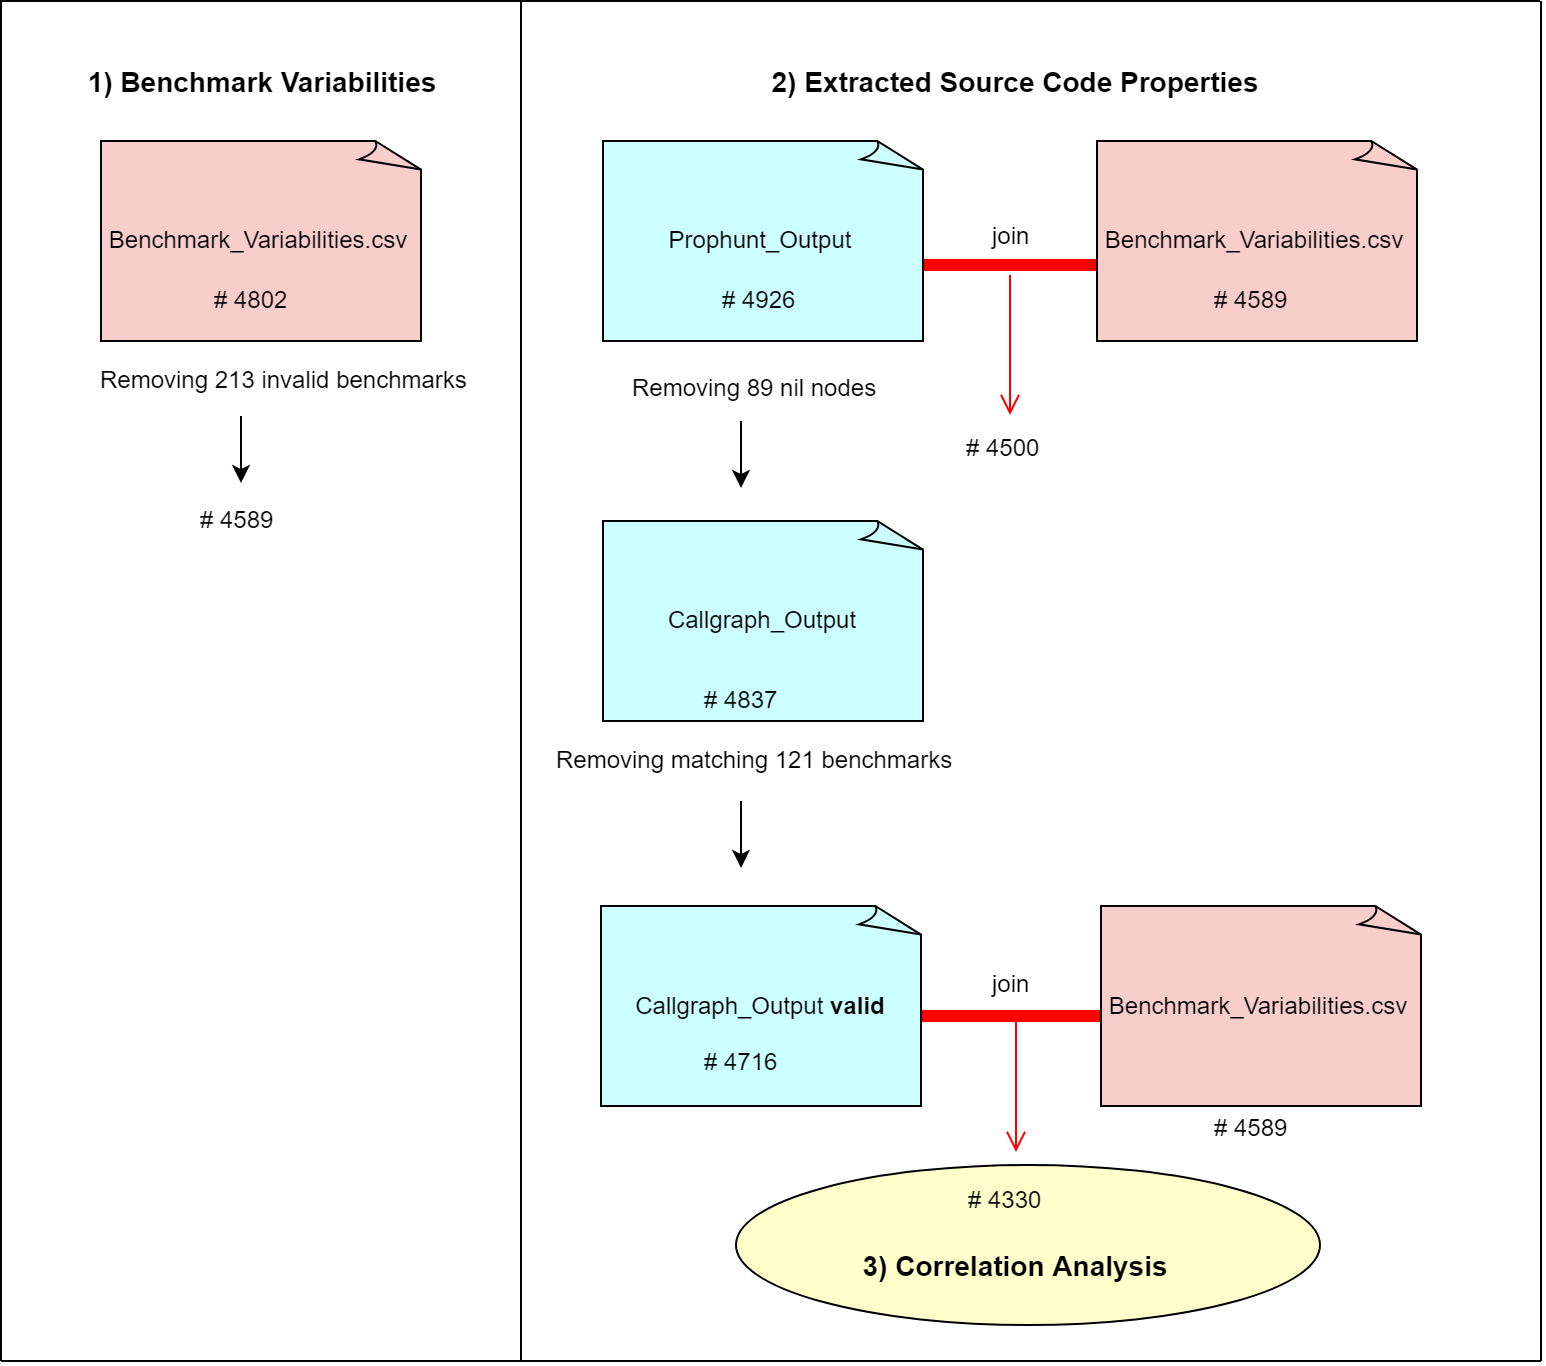
\includegraphics[width=\linewidth]{ResultsGeneral}
	\caption{General view of processing results.}
	\label{fig:results}
\end{figure}

\section{Variabilities of benchmarks}
\label{Variabilities of benchmarks}

In Section \ref{Analyzing variabilities}, I show which steps I go through to get variabilities of benchmarks, and in Section \ref{Benchmark Variabilities} I show the structure of \textbf{Benchmark\_Variabilities.csv}, which lists all the benchmarks from 230 projects. In total, there are 4802 benchmarks resulting from 230 projects. A quick investigation of this data shows that there are 204 benchmarks with only 1 execution, i.e. having only the average execution time of 1 benchmark iteration. Under these benchmarks are all the benchmarks of \textbf{mesos/mesos-go} \cite{mesos/mesos-go} and \textbf{go-gl/mathgl} \cite{go-gl/mathgl}, as well as benchmarks \textit{BenchmarkProtocolV2Sub128k} and \textit{BenchmarkCallsConcurrentServer} of projects \textbf{nsqio/nsq} \cite{nsqio/nsq} and \textbf{uber/tchannel-go} \cite{uber/tchannel-go}, respectively. Furthermore, there are in total 9 benchmarks, which, although having more than 1 execution, have a mean of 0, which in further investigation shows that all their execution times are 0 ns. Since having only 1 execution of a benchmark and having 0 ns as a mean execution time lead to not being able to calculate the standard derivation and RCIW values, I drop these benchmarks out of the \textbf{Benchmark\_Variabilities.csv} file, having left with 4589 benchmarks in total. The count of removed benchmarks and their belonging projects can be seen in Table \ref{removal1}.

\begin{table}[H]
\begin{longtable}[c]{@{}lcr@{}}
	\caption{Removal of invalid benchmarks from Benchmark\_Variabilities.csv.}
	\label{removal1}\\
	\toprule
	Project Name & Benchmark Count & Reason of Removal \\* \midrule
	\endfirsthead
	%
	\endhead
	%
	\bottomrule
	\endfoot
	%
	\endlastfoot
	%
	mesos/mesos-go & 178 & Benchmarks have only 1 iteration. \\
	go-gl/mathgl & 24 & Benchmarks have only 1 iteration. \\
	nsqio/nsq & 1 & Benchmark has only 1 iteration. \\
	uber/tchannel-go & 1 & Benchmark has only 1 iteration. \\
	prometheus/common & 1 & All counters are 0 ns. \\
	codegangsta/martini-contrib & 2 & All counters are 0 ns. \\
	DNAProject/DNA & 3 & All counters are 0 ns. \\
	TuftsBCB/io & 1 & All counters are 0 ns. \\
	cgrates/cgrates & 2 & All counters are 0 ns. \\* \bottomrule
\end{longtable}
\end{table}

\noindent For a general view of data, I create a histograms and density plots of benchmarks' variabilities using Matplotlib library \cite{Matplotlib} and Seaborn library\cite{Seaborn}, which are libraries for Python used often for visualizing data. For looking at the results on a project basis, I create tables for projects and report how many of projects fall into which bucket in terms of distribution of variabilities.

\subsection{Variabilities on benchmark level}

Figure \ref{fig:density1} shows the density distribution of all benchmarks found in \textbf{Benchmark\_Variabilities.csv} with all 3 variability metrics considered. According to this plot, most of the benchmarks are found between 0-10\%, however, the decrease of different metrics slightly differ from each other.

\begin{figure}[H]
	\centering
	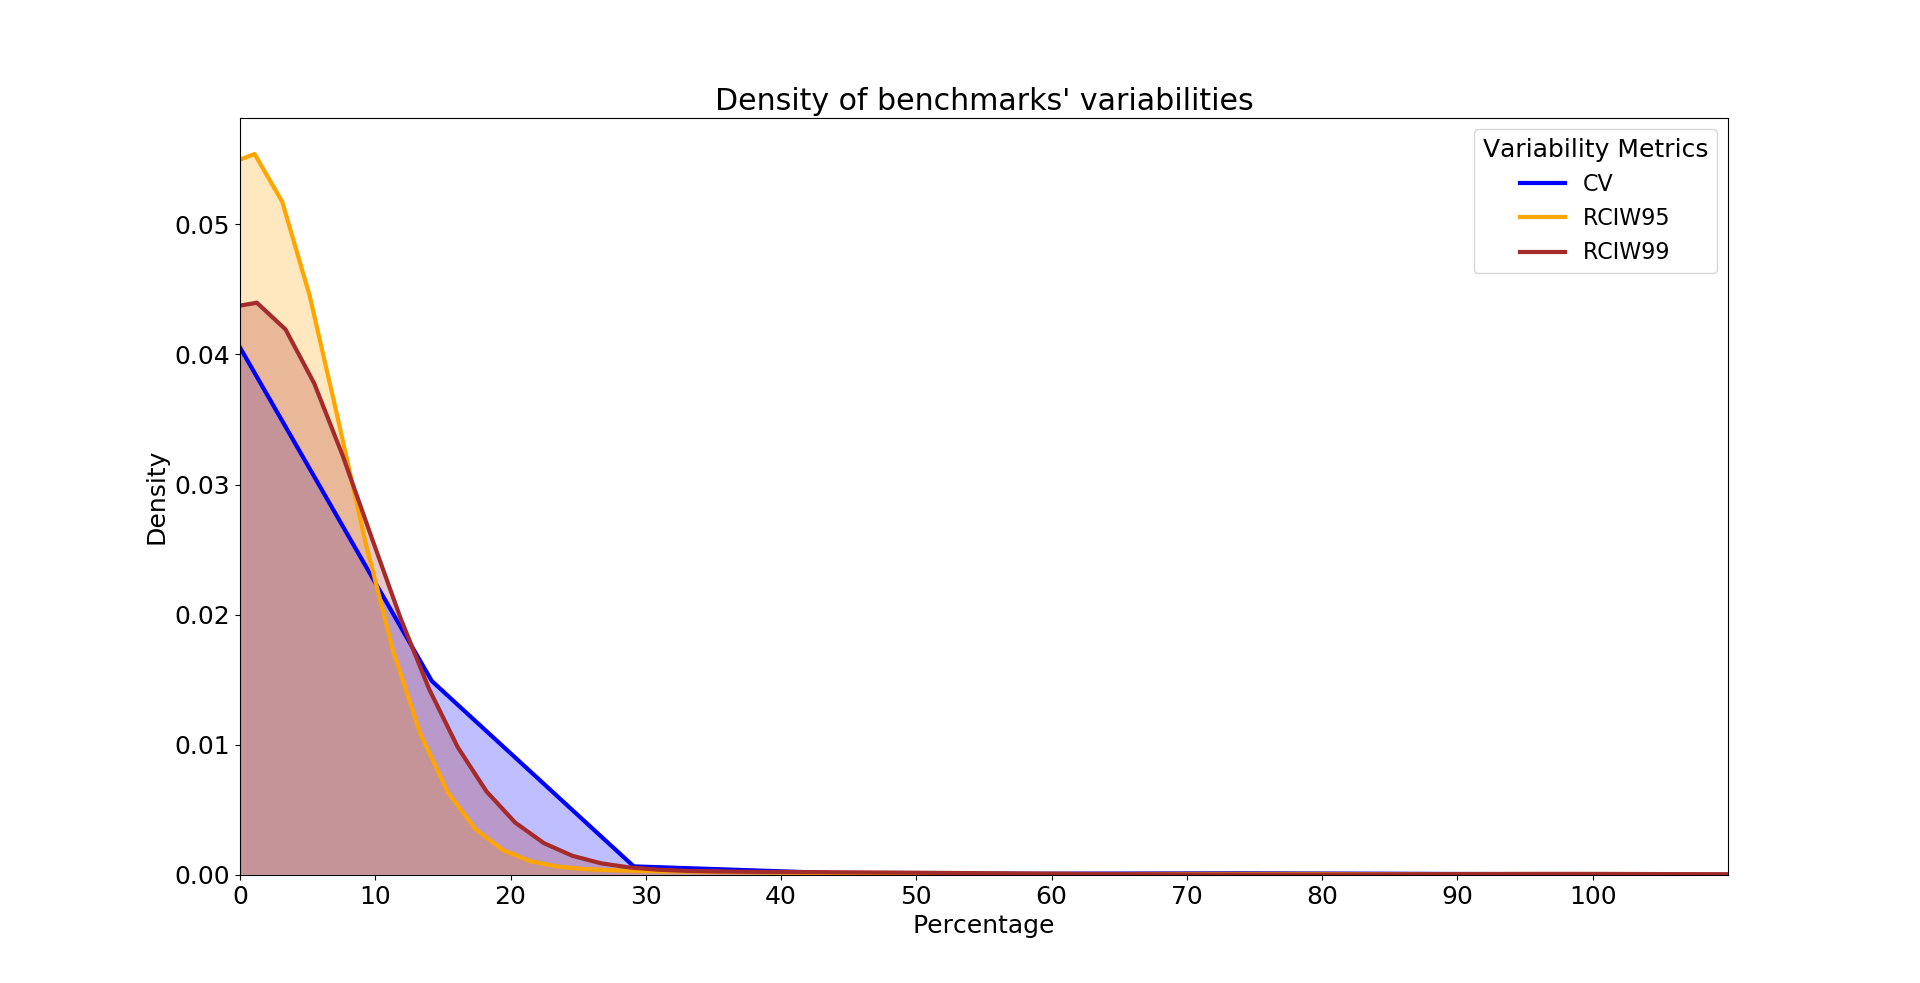
\includegraphics[width=\linewidth]{resultsvis/density_controlled1}
	\caption{Density of benchmarks' variabilities 1-100\%.}
	\label{fig:density1}
\end{figure}

\noindent Figure \ref{fig:log1} shows the histogram across all benchmarks and distributions of their variabilities in 10 percent buckets, taking all 3 metrics into consideration. According to the distribution, (CV) 97.50\% (4474/4589), (RCIW95) 98.48\% (4519/4589) and (RCIW99) 98.17\% (4505/4589) of all benchmarks have a variation between 0 and 10 percent. These are quite high percentages to tell that most of the benchmarks are very stable. Note that last bucket is for all the benchmarks that have a variation equal or higher than 100.

\begin{figure}[H]
	\centering
	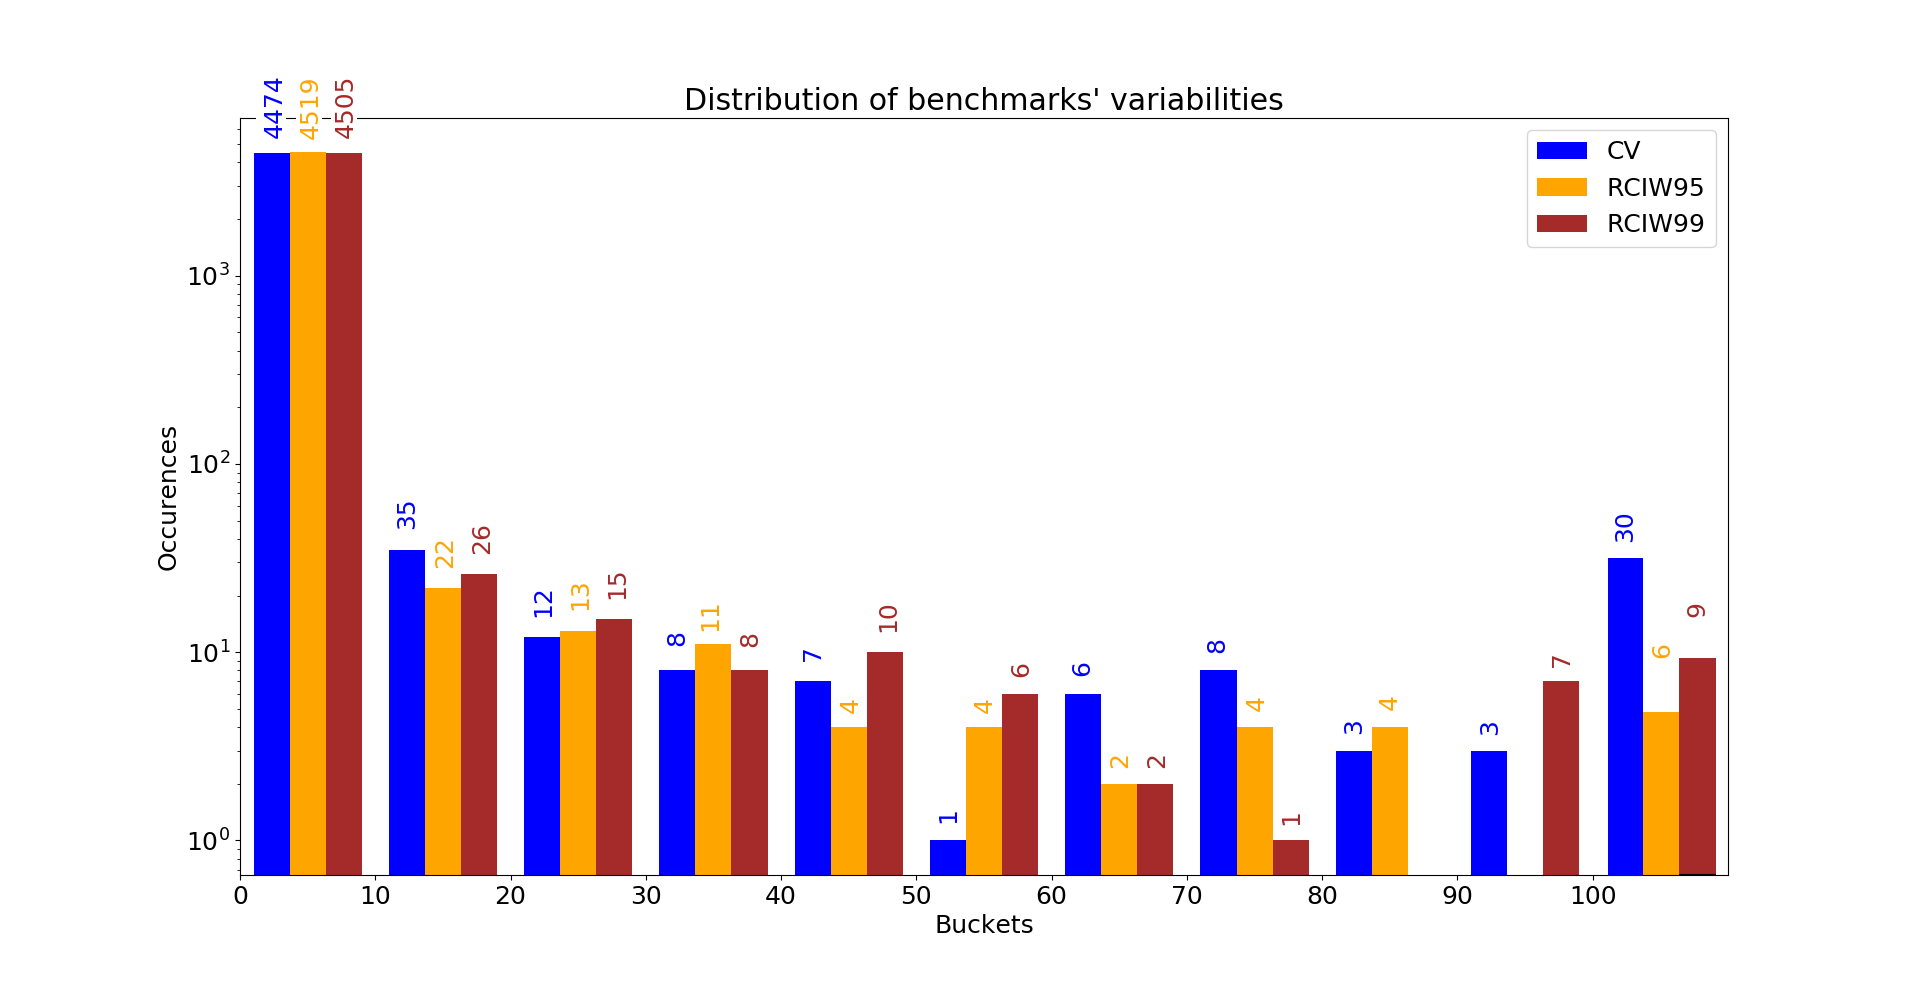
\includegraphics[width=\linewidth]{resultsvis/log1}
	\caption{Distribution of benchmarks' variabilities 0-100 in 10\% buckets.}
	\label{fig:log1}
\end{figure}

\noindent This result requires further analysis of the benchmarks in the 0-10\% bucket, and I create a second density plot showing this range in Figure \ref{fig:density2}. Although this time the decrease is not as sharp as in Figure \ref{fig:density1}, most of the variabilities fall in the range 0-1\%, which can be seen with numbers in the Figure \ref{fig:log2}.

\begin{figure}[H]
	\centering
	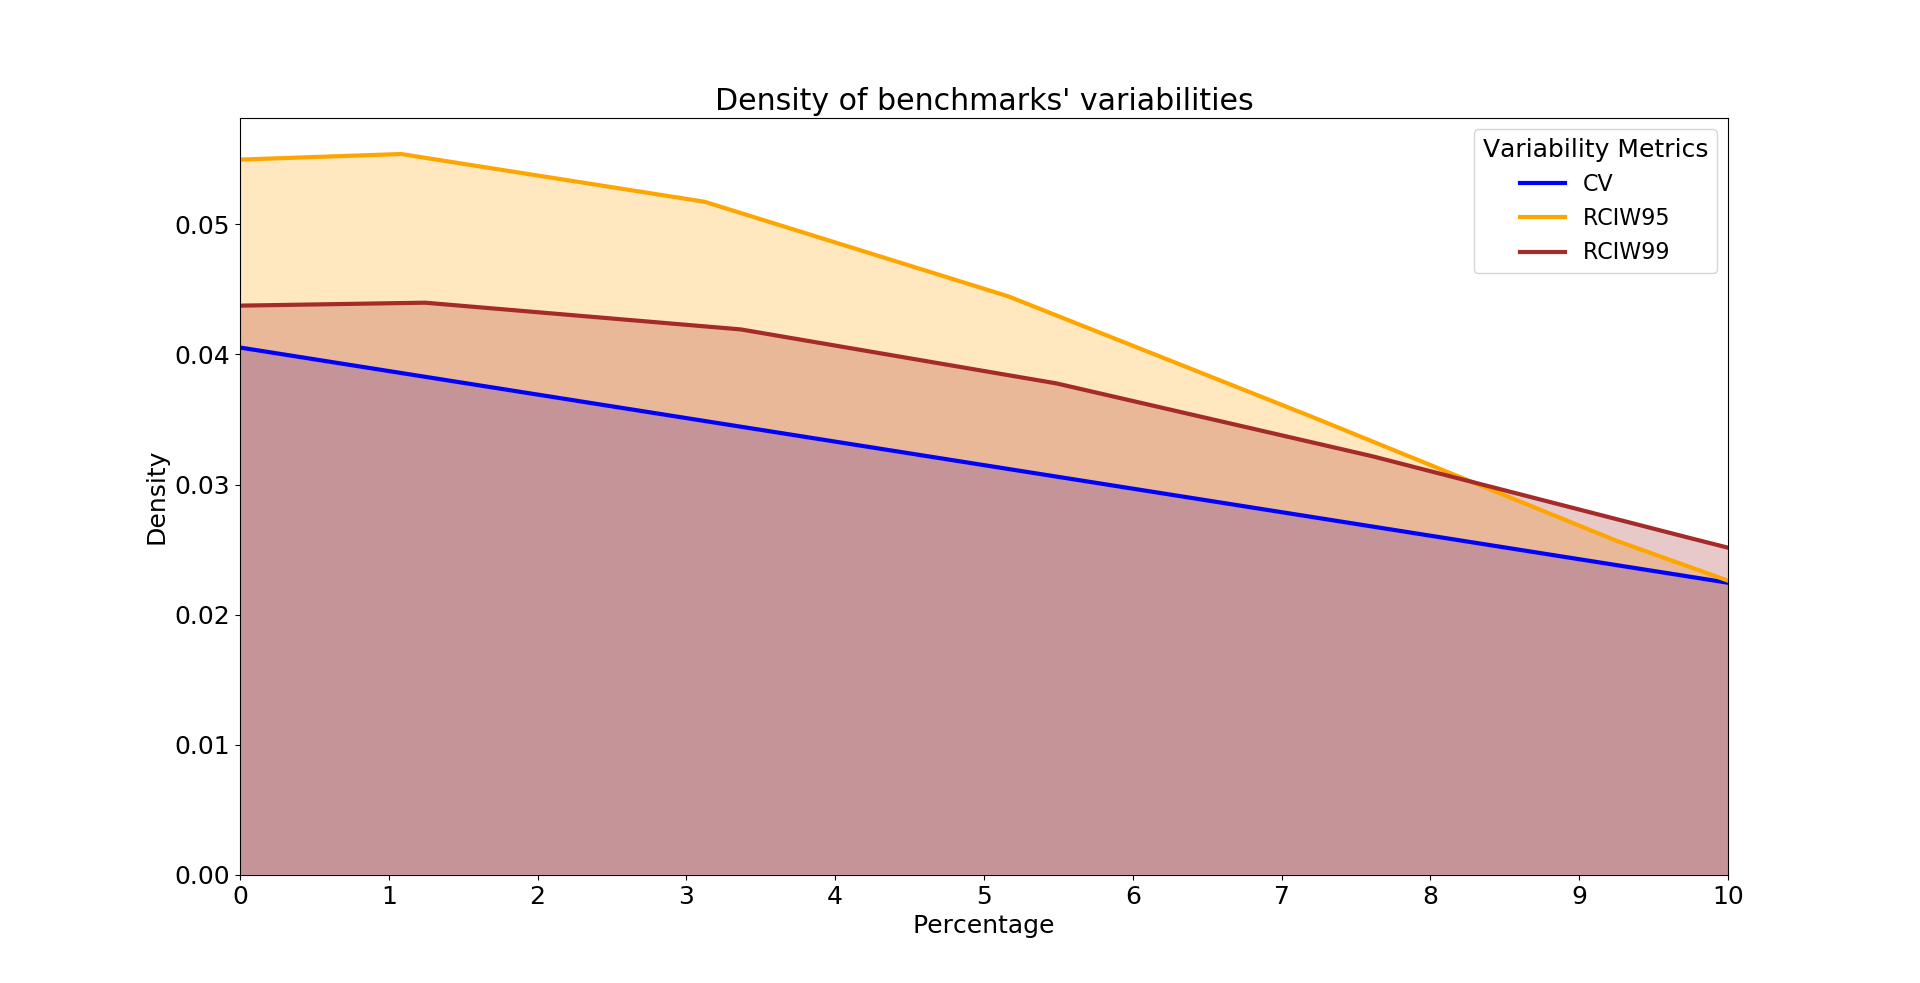
\includegraphics[width=\linewidth]{resultsvis/density_controlled2}
	\caption{Density of benchmarks' variabilities in 1-10\%.}
	\label{fig:density2}
\end{figure}

Figure \ref{fig:log2} exposes the variabilities in percentage. Most of the benchmarks fall into the bucket 0-1\%, building (CV) 81.74\% (3657/4474), (RCIW95) 89.20\% (4035/4519) and (RCIW99) 87.70\% (3951/4505) of the projects that are in the 1-10\% bucket. Although not as high in percentage as in 0-10\% bucket, most of the benchmarks can still be described as very stable, having a variation between 0 and 1 \%.

\begin{figure}[H]
	\centering
	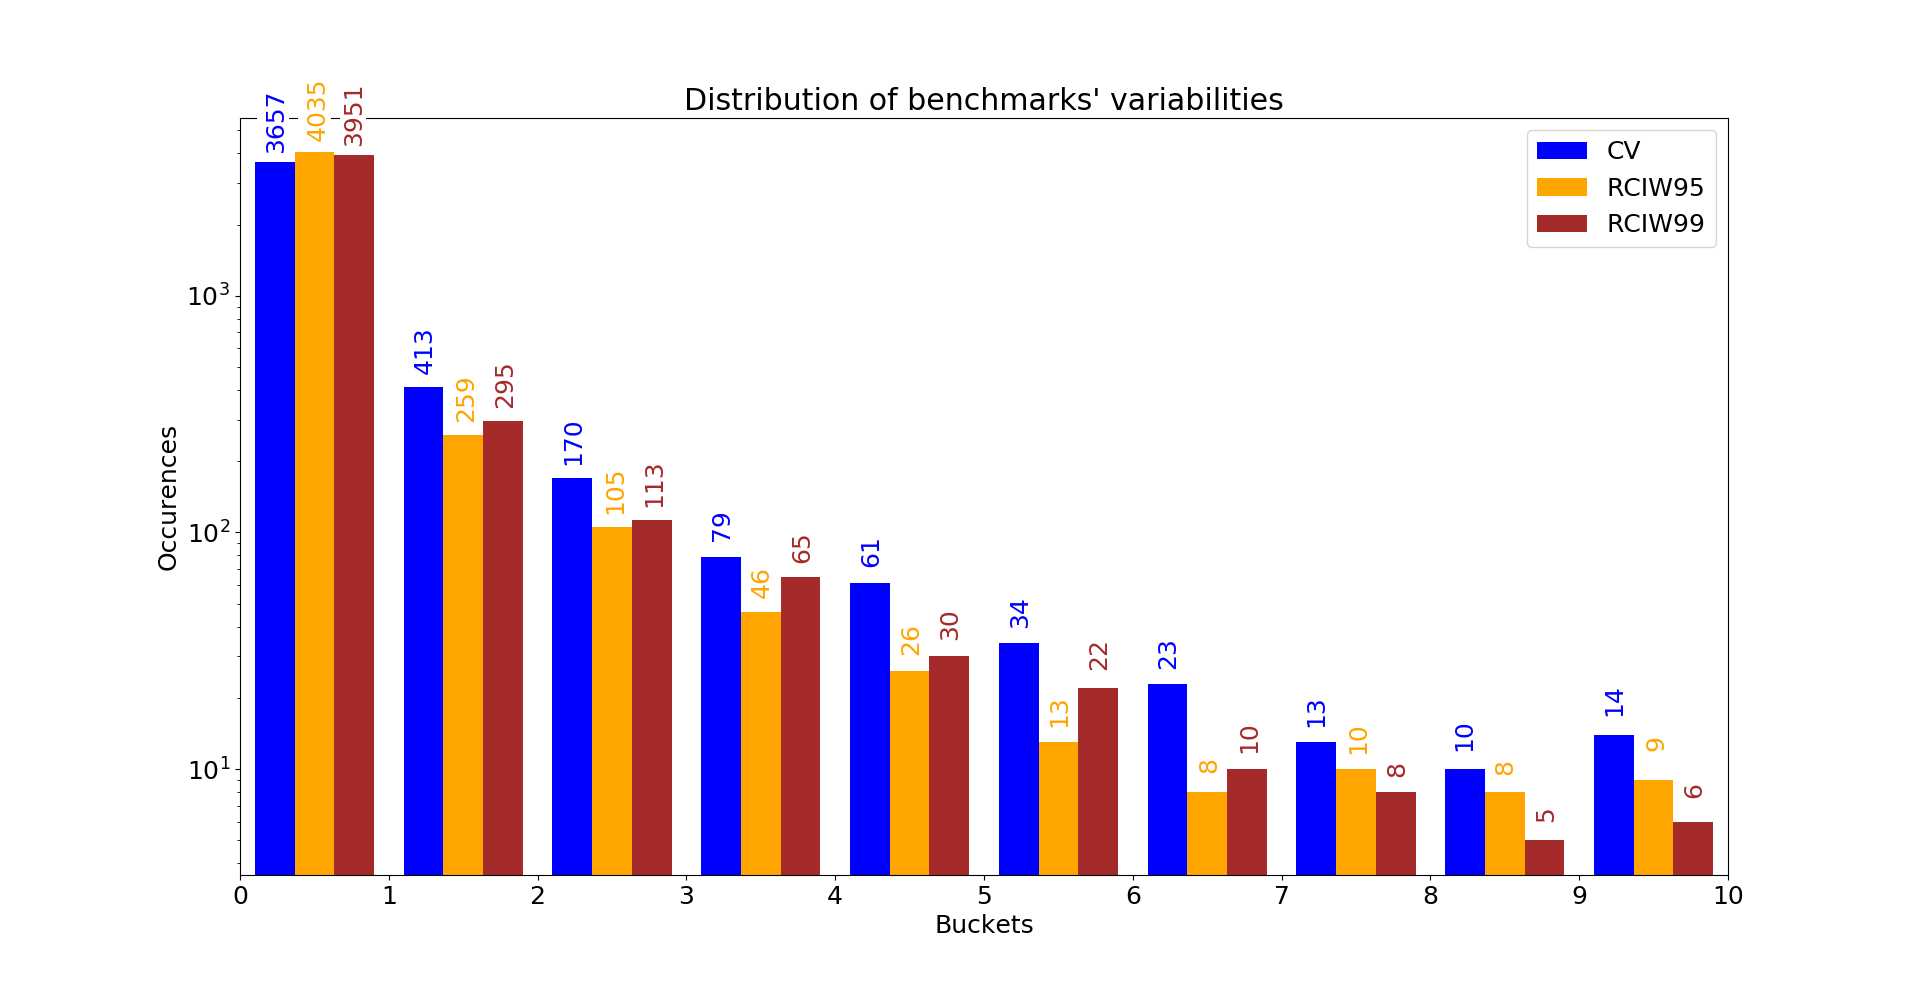
\includegraphics[width=\linewidth]{resultsvis/log2}
	\caption{Distribution of benchmarks' variabilities 0-10 in 1\% buckets.}
	\label{fig:log2}
\end{figure}

\subsection{Variabilities on project level}

Since I eliminate 2 projects because they have 1 execution for each of their benchmarks, following statistical data is based on a total of 228 projects. Table \ref{table:table1}'s header shows \textbf{Percentages} as buckets for the benchmarks' RCIW99 values. Following two rows show how many distinct projects fall into this group (i.e., having at least one benchmark in this bucket), and how many of the total projects this makes in percentage. As one can see, 225 out of 228 projects have benchmarks that have at least one benchmark that has a RCIW99 value between 0-1\%. Analyzing the 0-1\% bucket further shows that there are in total 283 benchmarks from 68 projects which have a RCIW99 value of 0.0\%. This makes 6.16\% of total benchmarks. A RCIW99 value of 0.0\% means that there is no variation in the results of the benchmark, which can be confirmed by looking at the iteration values of these benchmarks. The number of iterations for these benchmarks varies from 4 to 1519 with an average of 97 iterations, and the average execution time in ns varies from 0.48 ns to 2930.0 ns, having an average of 140 ns. Generally, the benchmarks that have 0.0\% of RCIW99 are short running benchmarks.

\begin{table}[H]
	\centering
	\caption{Number of distinct projects, whose benchmarks’ RCIW99 lay between 1-10\% in 1\% buckets and between 10-100\% in 10\% buckets}
	\label{table:table1}
	\resizebox{\textwidth}{!}{
	\begin{tabular}{lllllllllll}
		\hline
		\rowcolor[HTML]{FFFC9E} 
		\multicolumn{1}{|l|}{\cellcolor[HTML]{FFFC9E}Percentages} & \multicolumn{1}{l|}{\cellcolor[HTML]{FFFC9E}0-1\%}   & \multicolumn{1}{l|}{\cellcolor[HTML]{FFFC9E}1-2\%}   & \multicolumn{1}{l|}{\cellcolor[HTML]{FFFC9E}2-3\%}   & \multicolumn{1}{l|}{\cellcolor[HTML]{FFFC9E}3-4\%}   & \multicolumn{1}{l|}{\cellcolor[HTML]{FFFC9E}4-5\%}   & \multicolumn{1}{l|}{\cellcolor[HTML]{FFFC9E}5-6\%}   & \multicolumn{1}{l|}{\cellcolor[HTML]{FFFC9E}6-7\%}   & \multicolumn{1}{l|}{\cellcolor[HTML]{FFFC9E}7-8\%}   & \multicolumn{1}{l|}{\cellcolor[HTML]{FFFC9E}8-9\%}    & \multicolumn{1}{l|}{\cellcolor[HTML]{FFFC9E}9-10\%}              \\ \hline
		\multicolumn{1}{|l|}{\#projects}                          & \multicolumn{1}{l|}{225}                             & \multicolumn{1}{l|}{75}                              & \multicolumn{1}{l|}{48}                              & \multicolumn{1}{l|}{30}                              & \multicolumn{1}{l|}{17}                              & \multicolumn{1}{l|}{15}                              & \multicolumn{1}{l|}{8}                               & \multicolumn{1}{l|}{6}                               & \multicolumn{1}{l|}{4}                                & \multicolumn{1}{l|}{5}                                           \\ \hline
		\multicolumn{1}{|l|}{\#projects \%}                       & \multicolumn{1}{l|}{99\%}                            & \multicolumn{1}{l|}{33\%}                            & \multicolumn{1}{l|}{21\%}                            & \multicolumn{1}{l|}{13\%}                            & \multicolumn{1}{l|}{7\%}                             & \multicolumn{1}{l|}{7\%}                             & \multicolumn{1}{l|}{4\%}                             & \multicolumn{1}{l|}{3\%}                             & \multicolumn{1}{l|}{2\%}                              & \multicolumn{1}{l|}{2\%}                                         \\ \hline
		&                                                      &                                                      &                                                      &                                                      &                                                      &                                                      &                                                      &                                                      &                                                       &                                                                  \\ \hline
		\rowcolor[HTML]{FFFC9E} 
		\multicolumn{1}{|l|}{\cellcolor[HTML]{FFFC9E}Percentages} & \multicolumn{1}{l|}{\cellcolor[HTML]{FFFC9E}10-20\%} & \multicolumn{1}{l|}{\cellcolor[HTML]{FFFC9E}20-30\%} & \multicolumn{1}{l|}{\cellcolor[HTML]{FFFC9E}30-40\%} & \multicolumn{1}{l|}{\cellcolor[HTML]{FFFC9E}40-50\%} & \multicolumn{1}{l|}{\cellcolor[HTML]{FFFC9E}50-60\%} & \multicolumn{1}{l|}{\cellcolor[HTML]{FFFC9E}60-70\%} & \multicolumn{1}{l|}{\cellcolor[HTML]{FFFC9E}70-80\%} & \multicolumn{1}{l|}{\cellcolor[HTML]{FFFC9E}80-90\%} & \multicolumn{1}{l|}{\cellcolor[HTML]{FFFC9E}90-100\%} & \multicolumn{1}{l|}{\cellcolor[HTML]{FFFC9E}\textgreater{}100\%} \\ \hline
		\multicolumn{1}{|l|}{\#projects}                          & \multicolumn{1}{l|}{18}                              & \multicolumn{1}{l|}{9}                               & \multicolumn{1}{l|}{6}                               & \multicolumn{1}{l|}{4}                               & \multicolumn{1}{l|}{4}                               & \multicolumn{1}{l|}{2}                               & \multicolumn{1}{l|}{1}                               & \multicolumn{1}{l|}{0}                               & \multicolumn{1}{l|}{3}                                & \multicolumn{1}{l|}{6}                                           \\ \hline
		\multicolumn{1}{|l|}{\#projects \%}                       & \multicolumn{1}{l|}{8\%}                             & \multicolumn{1}{l|}{4\%}                             & \multicolumn{1}{l|}{3\%}                             & \multicolumn{1}{l|}{2\%}                             & \multicolumn{1}{l|}{2\%}                             & \multicolumn{1}{l|}{1\%}                             & \multicolumn{1}{l|}{0\%}                             & \multicolumn{1}{l|}{0\%}                             & \multicolumn{1}{l|}{1\%}                              & \multicolumn{1}{l|}{3\%}                                         \\ \hline
	\end{tabular}
	}
\end{table}

\noindent Table \ref{table:table2} similarly shows the number of projects and their percentages across all projects, whose benchmarks have an RCIW99 score of more than the one provided in the \textbf{Percentage} header. One thing that attracts attention is that in the first row there are 227 projects which have at least one benchmark that has a RCIW99 score bigger than 0. This is because one of the projects, \textbf{qjpcu/sesh} \cite{qjpcu/sesh}, only has 2 benchmarks, of which both have 0.0 as RCIW99 score.

\begin{table}[H]
	\centering
	\caption{Number of distinct projects, whose benchmarks’ RCIW99 lay more than the percent value}
	\label{table:table2}
	\begin{tabular}{lllllllllll}
		\hline
		\rowcolor[HTML]{FFCCC9} 
		\multicolumn{1}{|l|}{\cellcolor[HTML]{FFCCC9}Percentage} & \multicolumn{1}{l|}{\cellcolor[HTML]{FFCCC9}0\%}  & \multicolumn{1}{l|}{\cellcolor[HTML]{FFCCC9}1\%}  & \multicolumn{1}{l|}{\cellcolor[HTML]{FFCCC9}2\%}  & \multicolumn{1}{l|}{\cellcolor[HTML]{FFCCC9}3\%}  & \multicolumn{1}{l|}{\cellcolor[HTML]{FFCCC9}4\%}  & \multicolumn{1}{l|}{\cellcolor[HTML]{FFCCC9}5\%}  & \multicolumn{1}{l|}{\cellcolor[HTML]{FFCCC9}6\%}  & \multicolumn{1}{l|}{\cellcolor[HTML]{FFCCC9}7\%}  & \multicolumn{1}{l|}{\cellcolor[HTML]{FFCCC9}8\%}  & \multicolumn{1}{l|}{\cellcolor[HTML]{FFCCC9}9\%}   \\ \hline
		\multicolumn{1}{|l|}{\#projects}                         & \multicolumn{1}{l|}{227}                          & \multicolumn{1}{l|}{98}                           & \multicolumn{1}{l|}{75}                           & \multicolumn{1}{l|}{58}                           & \multicolumn{1}{l|}{47}                           & \multicolumn{1}{l|}{53}                           & \multicolumn{1}{l|}{39}                           & \multicolumn{1}{l|}{35}                           & \multicolumn{1}{l|}{32}                           & \multicolumn{1}{l|}{31}                            \\ \hline
		\multicolumn{1}{|l|}{\#projects \%}                      & \multicolumn{1}{l|}{100\%}                        & \multicolumn{1}{l|}{43\%}                         & \multicolumn{1}{l|}{33\%}                         & \multicolumn{1}{l|}{25\%}                         & \multicolumn{1}{l|}{21\%}                         & \multicolumn{1}{l|}{23\%}                         & \multicolumn{1}{l|}{17\%}                         & \multicolumn{1}{l|}{15\%}                         & \multicolumn{1}{l|}{14\%}                         & \multicolumn{1}{l|}{14\%}                          \\ \hline
		&                                                   &                                                   &                                                   &                                                   &                                                   &                                                   &                                                   &                                                   &                                                   &                                                    \\ \hline
		\rowcolor[HTML]{FFCCC9} 
		\multicolumn{1}{|l|}{\cellcolor[HTML]{FFCCC9}Percentage} & \multicolumn{1}{l|}{\cellcolor[HTML]{FFCCC9}10\%} & \multicolumn{1}{l|}{\cellcolor[HTML]{FFCCC9}20\%} & \multicolumn{1}{l|}{\cellcolor[HTML]{FFCCC9}30\%} & \multicolumn{1}{l|}{\cellcolor[HTML]{FFCCC9}40\%} & \multicolumn{1}{l|}{\cellcolor[HTML]{FFCCC9}50\%} & \multicolumn{1}{l|}{\cellcolor[HTML]{FFCCC9}60\%} & \multicolumn{1}{l|}{\cellcolor[HTML]{FFCCC9}70\%} & \multicolumn{1}{l|}{\cellcolor[HTML]{FFCCC9}80\%} & \multicolumn{1}{l|}{\cellcolor[HTML]{FFCCC9}90\%} & \multicolumn{1}{l|}{\cellcolor[HTML]{FFCCC9}100\%} \\ \hline
		\multicolumn{1}{|l|}{\#projects}                         & \multicolumn{1}{l|}{28}                           & \multicolumn{1}{l|}{18}                           & \multicolumn{1}{l|}{13}                           & \multicolumn{1}{l|}{10}                           & \multicolumn{1}{l|}{8}                            & \multicolumn{1}{l|}{6}                            & \multicolumn{1}{l|}{6}                            & \multicolumn{1}{l|}{6}                            & \multicolumn{1}{l|}{6}                            & \multicolumn{1}{l|}{6}                             \\ \hline
		\multicolumn{1}{|l|}{\#projects \%}                      & \multicolumn{1}{l|}{12\%}                         & \multicolumn{1}{l|}{8\%}                          & \multicolumn{1}{l|}{6\%}                          & \multicolumn{1}{l|}{4\%}                          & \multicolumn{1}{l|}{4\%}                          & \multicolumn{1}{l|}{3\%}                          & \multicolumn{1}{l|}{3\%}                          & \multicolumn{1}{l|}{3\%}                          & \multicolumn{1}{l|}{3\%}                          & \multicolumn{1}{l|}{3\%}                           \\ \hline
	\end{tabular}
\end{table}

\noindent If we call the benchmarks which have a RCIW99 value above 60\% unstable benchmarks, then there are in total 19 benchmarks from 6 projects which are unstable. Table \ref{table:unstable} shows in detail the RCIW99 values of benchmarks, their projects, and the commit they are from.

\begin{table}[H]
\begin{longtable}[c]{@{}lll@{}}
	\caption{Unstable benchmarks}
	\label{unstable}\\
	\toprule
	Project Name & Benchmark & RCIW99 \\* \midrule
	\endfirsthead
	%
	\endhead
	%
	\bottomrule
	\endfoot
	%
	\endlastfoot
	%
	tendermint/go-merkle & /benchmarks/bench\_test.go/BenchmarkLevelDBBatchSizes & 101.90618356378155 \\
	tendermint/go-merkle & /benchmarks/bench\_test.go/BenchmarkMedium & 97.90949382723956 \\
	tendermint/go-merkle & /benchmarks/bench\_test.go/BenchmarkRandomBytes & 99.07987400530504 \\
	tendermint/go-merkle & /benchmarks/bench\_test.go/BenchmarkSmall & 96.8579891360519 \\
	tendermint/merkleeyes & /benchmarks/bench\_test.go/BenchmarkLevelDBBatchSizes & 98.59817524979992 \\
	tendermint/merkleeyes & /benchmarks/bench\_test.go/BenchmarkMedium & 93.97081845239374 \\
	tendermint/merkleeyes & /benchmarks/bench\_test.go/BenchmarkMemKeySizes & 63.065558656556966 \\
	tendermint/merkleeyes & /benchmarks/bench\_test.go/BenchmarkRandomBytes & 111.31606792006772 \\
	tendermint/merkleeyes & /benchmarks/bench\_test.go/BenchmarkSmall & 96.49370081581276 \\
	xtaci/kcp-go & sess\_test.go/BenchmarkSinkSpeed1M & 79.15061748312237 \\
	xtaci/kcp-go & sess\_test.go/BenchmarkSinkSpeed256K & 170.19650415760373 \\
	xtaci/kcp-go & sess\_test.go/BenchmarkSinkSpeed4K & 90.76953191237926 \\
	xtaci/kcp-go & sess\_test.go/BenchmarkSinkSpeed64K & 133.5089191240669 \\
	uber/tchannel-go & relay\_benchmark\_test.go/BenchmarkRelayNoLatencies & 196.25602170651797 \\
	micro/go-micro & /broker/http\_broker\_test.go/BenchmarkPub128 & 140.02193180903242 \\
	micro/go-micro & /transport/http/http\_test.go/BenchmarkTransport1 & 121.92430559307232 \\
	segmentio/objconv & /cbor/cbor\_test.go/BenchmarkCodec & 204.0738989031456 \\
	segmentio/objconv & /json/json\_test.go/BenchmarkCodec & 188.40021466179115 \\
	segmentio/objconv & /objutil/int\_test.go/BenchmarkParseUintHex & 64.18111561234029 \\* \bottomrule
\end{longtable}
\end{table}

\noindent As I present the results for the first step of my methodology, I want to remind and answer the following research question:

\begin{itemize}
	\item \textbf{RQ1: How variable are microbenchmark results of Go projects?}
\end{itemize}

\noindent Unlike my hypothesis, there is no normalized distribution of RCIW99 values of benchmarks. Most of the benchmarks fall to the bucket 1-10\% (98.17\%), from which again most them fall to 0-1\% (87.70\%). Based on the dataset that I analyze with 230 projects, it is clear that most of them are very stable, and 6.16\% (283 in total) of benchmarks don't even vary, i.e., for each execution they have the same amount of nanoseconds as execution time. On the other side, 19 benchmarks from 6 projects are rather unstable with a RCIW99 above 60\%, which makes only 0.4\% of all the benchmarks. The possible reasons for the stability of benchmarks, as well as why there is such a distribution is furthermore discussed in the \ref{Discussion}. Section.


\section{Extracted source code features}
\label{Extracted source code features}

\subsection{Downloaded Projects}
Using all the 228 projects and their commits from the first results, my Python downloader script is able to download 223 of the projects successfully. From the remaining 5 projects, 3 (\textbf{tendermint/go-merkle}, \textbf{pp2p/paranoid}, \textbf{eleme/banshee}) are not found, either because they terminated the project on Github, or because they moved the project to another repository within or out of Github. 1 project (\textbf{stratumn/sdk} \cite{stratumn/sdk}) changed its repo and its redirection from Github results in a non-Go-project. 1 project (\textbf{eaburns/T}) changed the repo to a new name (\textbf{eaburns/T\_old}) \cite{eaburns/T_old}, however, it's commit from the initial dataset does not match any commits in the new repo.\\
\\
As described in Section \ref{Prophunt} and \ref{Callgraph Analyzer}, parsing with Prophunt results with Prophunt\_Output and using the Callgraph Analyzer results with Callgraph\_Output. Prior to running both of the tools, I set up a Virtual Machine for Ubuntu 18.04 in my Windows 10 installation, because some projects have dependencies to some standard library packages, which are not included in a Windows installation of Go, such as "syscall". Not having such libraries causes compilation errors for some projects, hence, I run both of the tools in Ubuntu. This ensures a smoother experience when parsing and extracting properties that rely on the standard library packages.\\

\subsection{Prophunt Output}

Prophunt returns in total 223 CSV files with a size of 35.2 MB. In total, Prophunt parses 163474 functions across all 223 projects. This makes an average of 733 functions per project, and Figure \ref{fig:parsed} illustrates the number of parsed functions per project on a log scaled y-axis. From this many functions, there are 4926 parsed benchmarks, which in average equals to 22 benchmarks per project. The frequency of parsed benchmarks per project is illustrated in Figure \ref{fig:parsedb}. This is more than the total number of benchmarks found in the Benchmark\_Variabilities.csv (4589) and means that the parser was able to find 337 more benchmarks than in the given dataset. However, when matching them with the benchmarks from Benchmark\_Variabilities.csv, there are in total 4500 matching benchmarks. That is explainable with the missing benchmarks from unsuccessfull downloads and some compilation problems in 2 projects albeit all dependency fetching efforts. In Table \ref{table:infinalnotcsv1} is the projects of benchmarks (89) that are present in Benchmark\_Variabilities.csv, yet could not be parsed with Prophunt (See in \ref{infinalbutnotincsv1}):\\


\begin{figure}[H]
	\centering
	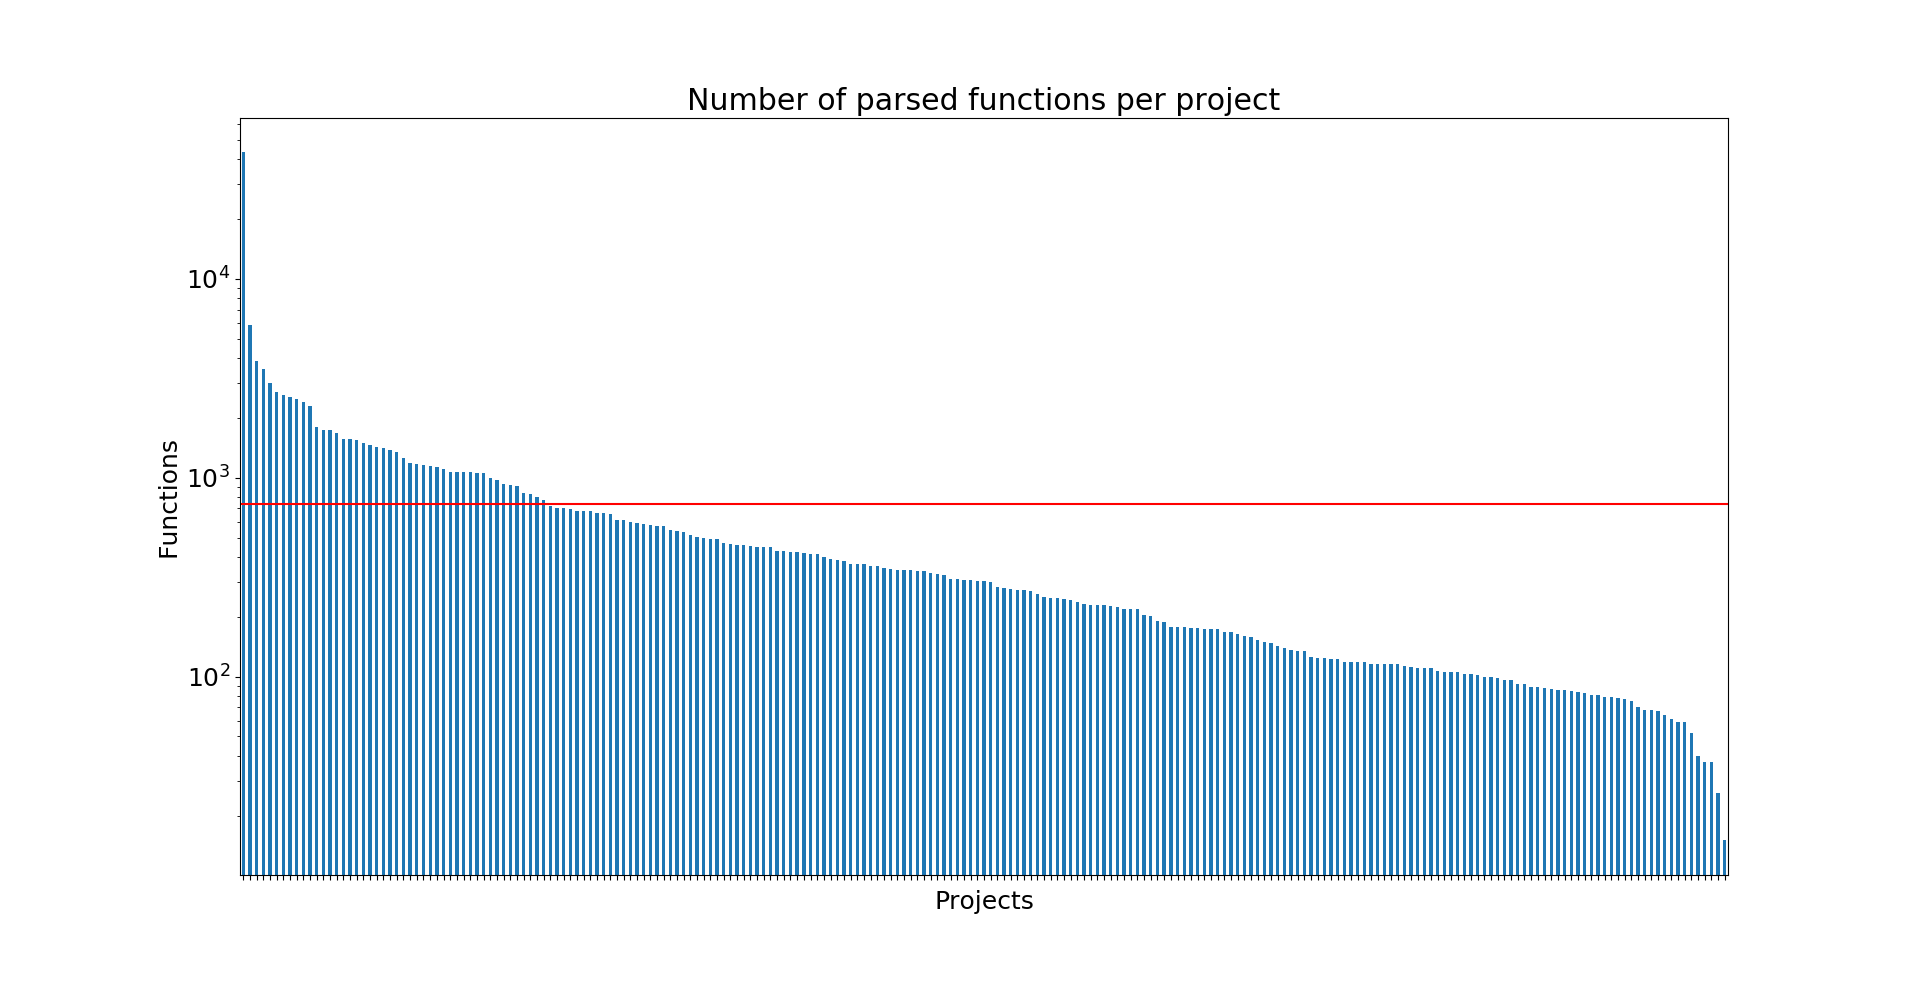
\includegraphics[width=\textwidth]{parsedfunctions}
	\caption{Number of parsed functions per project.}
	\label{fig:parsed}
\end{figure}

\begin{figure}[H]
	\centering
	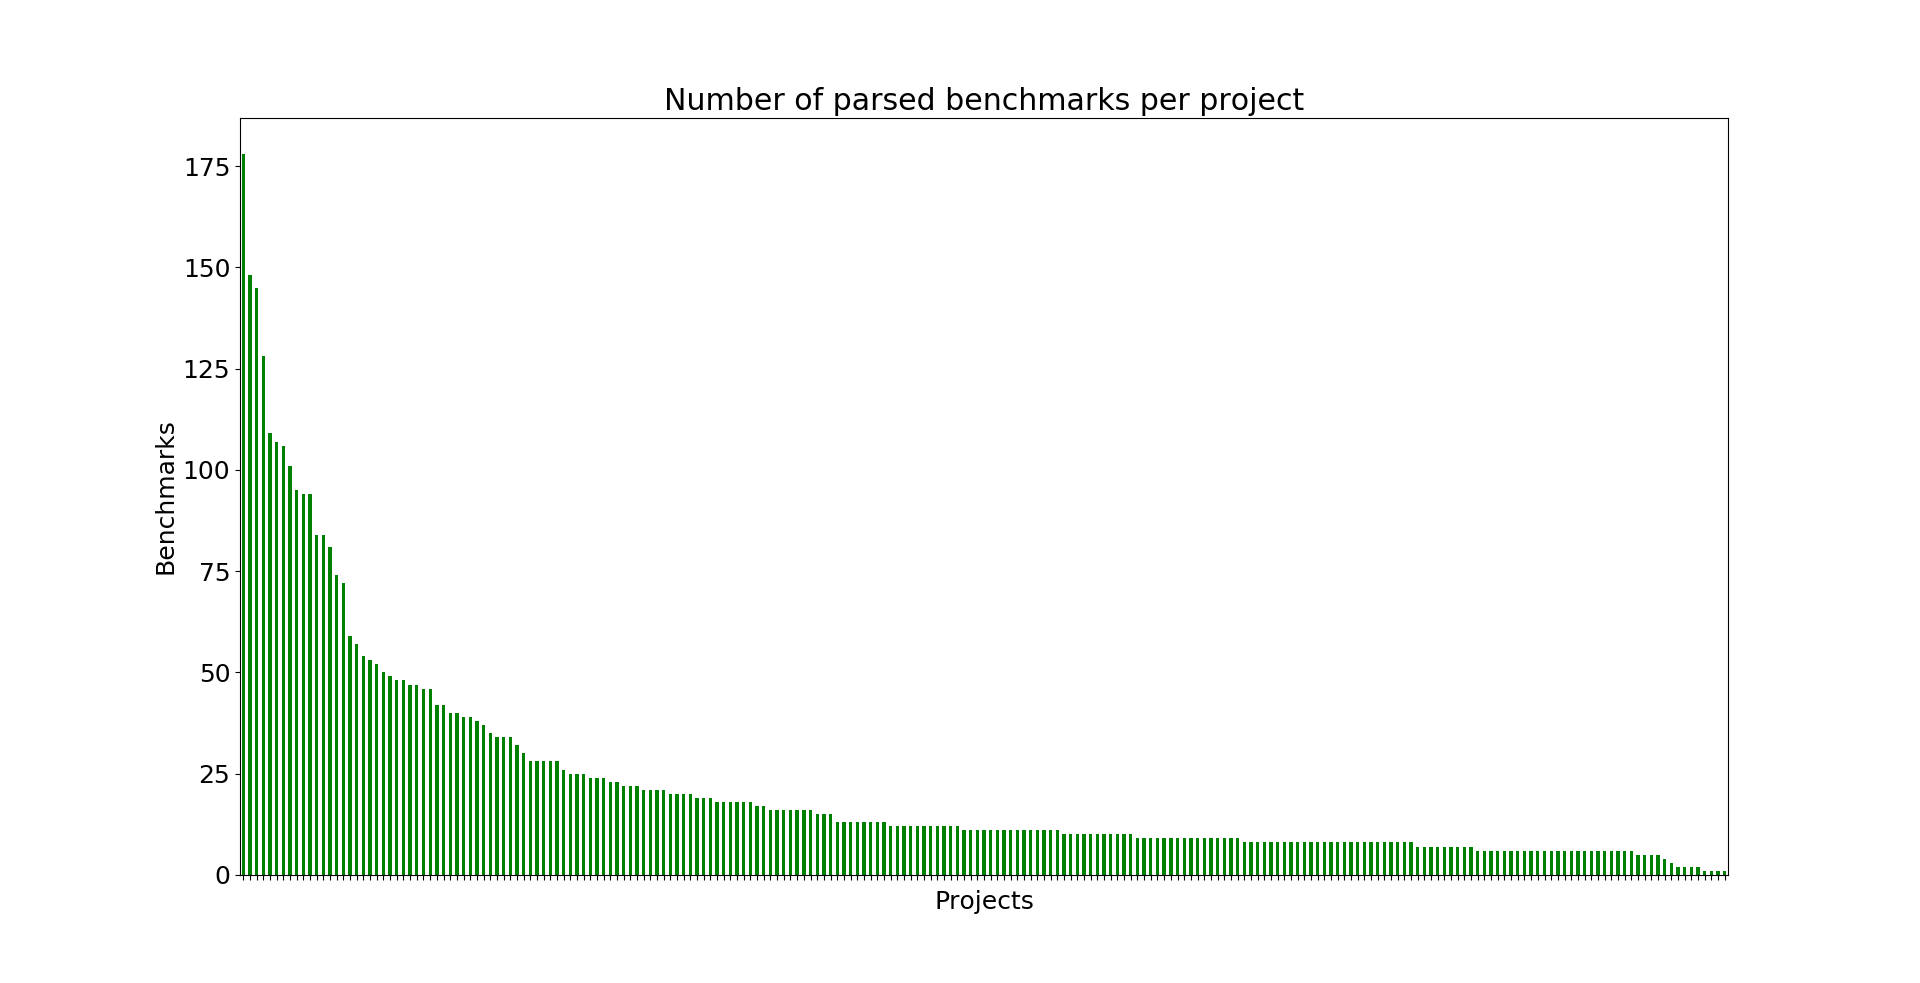
\includegraphics[width=\textwidth]{parsedbenchmarks}
	\caption{Number of parsed benchmarks per project.}
	\label{fig:parsedb}
\end{figure}


\begin{table}
\begin{longtable}[c]{@{}lll@{}}
	\caption{Information about projects of not matching benchmarks}
	\label{table:infinalnotcsv1}\\
	\toprule
	Project Name & Benchmark Count & Reason of not match \\* \midrule
	\endfirsthead
	%
	\endhead
	%
	\bottomrule
	\endfoot
	%
	\endlastfoot
	%
	tendermint/go-merkle & 6 & Not found \\
	pp2p/paranoid & 14 & Not found \\
	eleme/banshee & 19 & Not found \\
	micro/go-micro & 10 & Not compiling \\
	coredns/coredns & 1 & Not compiling \\
	stratumn/sdk & 2 & Changed repo \\
	eaburns/T & 37 & Changed repo \\* \bottomrule
\end{longtable}
\end{table}


\subsection{Callgraph Analyzer Output}
Callgraph Analyzer takes as input the CSV files that are found in Prophunt\_Output. I run Callgraph Analyzer and collect 223 CSV files again. The valid 223 CSV files size up to 1.38 MB, with a total of 4837 benchmarks. This shows that 89 of the benchmarks in Prophunt\_Output were not analyzed via Callgraph Analyzer, because they had a nil node in the \textbf{*simple.DirectedGraph} instance of the project (See in \ref{incsv1butnotincsv2}). In the next step, I compare the benchmarks from Prophunt\_Output with the ones from Callgraph\_Output to see whether any benchmark has exactly same property values in both of the versions, and I find 121 exact same benchmarks (See in\ref{sameincsv1asincsv2}). This indicates that Callgraph Analyzer could not find any reachable node from these benchmarks, hence, it took the existing version of benchmark entry from Prophunt\_Output to Callgraph\_Output. For the sake of proper analysis, I eliminate these 121 benchmarks from Callgraph\_Output, having left with 4716 valid benchmarks and their properties.\\
\\
Finally, I match the benchmarks from Benchmark\_Variabilities.csv with the valid ones from Callgraph\_Output and see that there are 4330 matching benchmarks. This means that in total there are 259 not matching benchmarks of which 89 were not present in Prophunt\_Output in first place. Rest of 170 benchmarks do not match due to *simple.DirectedGraph not giving any reachable node, or callgraph tool cannot find the benchmark in the folders. 


\section{Correlation between variabilities and source code properties}
\label{Correlation results}

Section \ref{Variabilities of benchmarks} and \ref{Extracted source code features} were preliminary steps to build the final dataset of benchmarks, which includes the variability metrics RCIW99, RCIW95, CV, as well as the 59 source code property values for each of the 4330 benchmarks. As stated in Section \ref{Correlation analysis}, the correlation analysis made on this thesis relies on Spearman's rank-order correlation coefficients. For better focus on different types of properties, I present the results in Subsections \ref{Language related properties} and \ref{Standard library related properties}. Because "parameters" and "net/http/httptrace" have 0 value across all benchmarks, there is no correlation found between them and the stability, hence, they are removed from the analysis.

\subsection{Language related properties}
\label{Language related properties}

There are in total 27 language related properties including "cyclomaticcomplexity" that are the part of this analysis. Table \ref{table:languageproperties} shows the correlation values of these properties with the according variability metric (a concatenating * means a p-value lower than 0.05, and ** means a p-value lower than 0.01).

\begin{table}[H]
	\centering
	\caption{Correlation between stability and language related properties.}
	\label{table:languageproperties}
	\begin{tabular}{@{}llll@{}}
		Property Name & rciw99 & rciw95 & cv \\
		\toprule
		pkgfiles & \cellcolor[HTML]{FFCC99}0.28000** & \cellcolor[HTML]{FFCC99}0.28310** & \cellcolor[HTML]{99CCFF}0.20296** \\
		fileloc & \cellcolor[HTML]{FFCC99}0.25547** & \cellcolor[HTML]{FFCC99}0.26357** & \cellcolor[HTML]{99CCFF}0.17676** \\
		namelength & \cellcolor[HTML]{99CCFF}0.10807** & \cellcolor[HTML]{99CCFF}0.11421** & \cellcolor[HTML]{3366FF}0.05583** \\
		returns & \cellcolor[HTML]{FFCC99}0.28535** & \cellcolor[HTML]{FFCC99}0.28778** & \cellcolor[HTML]{C0C0C0}0.22448** \\
		loc & \cellcolor[HTML]{C0C0C0}0.24654** & \cellcolor[HTML]{C0C0C0}0.24957** & \cellcolor[HTML]{99CCFF}0.19555** \\
		funccalls & \cellcolor[HTML]{C0C0C0}0.25208** & \cellcolor[HTML]{FFCC99}0.25542** & \cellcolor[HTML]{99CCFF}0.20048** \\
		loops & \cellcolor[HTML]{C0C0C0}0.23889** & \cellcolor[HTML]{C0C0C0}0.24372** & \cellcolor[HTML]{99CCFF}0.18443** \\
		nestedloops & \cellcolor[HTML]{99CCFF}0.18190** & \cellcolor[HTML]{99CCFF}0.18672** & \cellcolor[HTML]{99CCFF}0.13891** \\
		channels & \cellcolor[HTML]{FFCC99}0.27211** & \cellcolor[HTML]{FFCC99}0.27868** & \cellcolor[HTML]{C0C0C0}0.23050** \\
		sends & \cellcolor[HTML]{C0C0C0}0.22830** & \cellcolor[HTML]{C0C0C0}0.23290** & \cellcolor[HTML]{99CCFF}0.18796** \\
		receives & \cellcolor[HTML]{C0C0C0}0.24083** & \cellcolor[HTML]{C0C0C0}0.24562** & \cellcolor[HTML]{99CCFF}0.19546** \\
		closes & \cellcolor[HTML]{FFCC99}0.26428** & \cellcolor[HTML]{FFCC99}0.27345** & \cellcolor[HTML]{99CCFF}0.21205** \\
		gos & \cellcolor[HTML]{FFCC99}0.28593** & \cellcolor[HTML]{FFCC99}0.29192** & \cellcolor[HTML]{C0C0C0}0.24832** \\
		concrranges & \cellcolor[HTML]{3366FF}0.04556** & \cellcolor[HTML]{3366FF}0.04388** & \cellcolor[HTML]{3366FF}0.03319* \\
		selects & \cellcolor[HTML]{C0C0C0}0.25025** & \cellcolor[HTML]{FFCC99}0.25777** & \cellcolor[HTML]{99CCFF}0.18467** \\
		selectcases & \cellcolor[HTML]{C0C0C0}0.25005** & \cellcolor[HTML]{FFCC99}0.25751** & \cellcolor[HTML]{99CCFF}0.18493** \\
		variables & \cellcolor[HTML]{C0C0C0}0.24846** & \cellcolor[HTML]{C0C0C0}0.25292** & \cellcolor[HTML]{99CCFF}0.20061** \\
		pointers & \cellcolor[HTML]{FFCC99}0.28430** & \cellcolor[HTML]{FFCC99}0.29096** & \cellcolor[HTML]{C0C0C0}0.22130** \\
		slices & \cellcolor[HTML]{99CCFF}0.17991** & \cellcolor[HTML]{99CCFF}0.18075** & \cellcolor[HTML]{99CCFF}0.13344** \\
		maps & \cellcolor[HTML]{99CCFF}0.17304** & \cellcolor[HTML]{99CCFF}0.17262** & \cellcolor[HTML]{99CCFF}0.16990** \\
		ifelses & \cellcolor[HTML]{C0C0C0}0.25134** & \cellcolor[HTML]{FFCC99}0.25509** & \cellcolor[HTML]{99CCFF}0.20447** \\
		switches & \cellcolor[HTML]{99CCFF}0.08179** & \cellcolor[HTML]{99CCFF}0.08671** & \cellcolor[HTML]{3366FF}0.04099** \\
		switchcases & \cellcolor[HTML]{99CCFF}0.07659** & \cellcolor[HTML]{99CCFF}0.08068** & \cellcolor[HTML]{3366FF}0.04293** \\
		panics & \cellcolor[HTML]{99CCFF}0.16285** & \cellcolor[HTML]{99CCFF}0.17181** & \cellcolor[HTML]{99CCFF}0.10483** \\
		recovers & \cellcolor[HTML]{3366FF}0.07039** & \cellcolor[HTML]{3366FF}0.06250** & \cellcolor[HTML]{99CCFF}0.07748** \\
		defers & \cellcolor[HTML]{FFCC99}0.27512** & \cellcolor[HTML]{FFCC99}0.27477** & \cellcolor[HTML]{C0C0C0}0.24704** \\
		cyclomaticcomplexity & \cellcolor[HTML]{FFCC99}0.25656** & \cellcolor[HTML]{FFCC99}0.26004** & \cellcolor[HTML]{99CCFF}0.20563** \\
		\bottomrule
	\end{tabular}
\end{table}

Taking RCIW99 correlations into consideration, the most correlating 3 properties are "gos", "returns" and "pointers" all with a very high significance. 

\subsection{Standard library related properties}
\label{Standard library related properties}

\begin{table}[H]
	\begin{tabular}{@{}llll@{}}
		property\_name & rciw99 & rciw95 & cv \\
		\toprule
		bufio & \cellcolor[HTML]{99CCFF}0.15467** & \cellcolor[HTML]{99CCFF}0.16217** & \cellcolor[HTML]{99CCFF}0.10351** \\
		bytes & \cellcolor[HTML]{99CCFF}0.16678** & \cellcolor[HTML]{99CCFF}0.16779** & \cellcolor[HTML]{99CCFF}0.15004** \\
		crypto & \cellcolor[HTML]{333399}\color{white}-0.02982* & \cellcolor[HTML]{333399}\color{white}-0.03062* & \cellcolor[HTML]{333399}\color{white}-0.02616 \\
		database/sql & \cellcolor[HTML]{333399}\color{white}0.01040 & \cellcolor[HTML]{333399}\color{white}0.00881 & \cellcolor[HTML]{333399}\color{white}-0.00608 \\
		encoding & \cellcolor[HTML]{99CCFF}0.12044** & \cellcolor[HTML]{99CCFF}0.11960** & \cellcolor[HTML]{99CCFF}0.07911** \\
		encoding/binary & \cellcolor[HTML]{99CCFF}0.08718** & \cellcolor[HTML]{99CCFF}0.09103** & \cellcolor[HTML]{3366FF}0.04150** \\
		encoding/csv & \cellcolor[HTML]{333399}\color{white}-0.00911 & \cellcolor[HTML]{333399}\color{white}-0.01151 & \cellcolor[HTML]{3366FF}0.01892 \\
		encoding/json & \cellcolor[HTML]{99CCFF}0.09332** & \cellcolor[HTML]{99CCFF}0.09174** & \cellcolor[HTML]{3366FF}0.06628** \\
		encoding/xml & \cellcolor[HTML]{3366FF}0.05489** & \cellcolor[HTML]{3366FF}0.05191** & \cellcolor[HTML]{3366FF}0.05730** \\
		io & \cellcolor[HTML]{99CCFF}0.20088** & \cellcolor[HTML]{99CCFF}0.20167** & \cellcolor[HTML]{99CCFF}0.15897** \\
		io/ioutil & \cellcolor[HTML]{99CCFF}0.17902** & \cellcolor[HTML]{99CCFF}0.18179** & \cellcolor[HTML]{99CCFF}0.13742** \\
		math & \cellcolor[HTML]{99CCFF}0.13606** & \cellcolor[HTML]{99CCFF}0.14590** & \cellcolor[HTML]{99CCFF}0.08024** \\
		math/rand & \cellcolor[HTML]{FFCC99}0.26986** & \cellcolor[HTML]{FFCC99}0.27009** & \cellcolor[HTML]{C0C0C0}0.22528** \\
		mime & \cellcolor[HTML]{99CCFF}0.14102** & \cellcolor[HTML]{99CCFF}0.14973** & \cellcolor[HTML]{99CCFF}0.11820** \\
		net & \cellcolor[HTML]{C0C0C0}0.23078** & \cellcolor[HTML]{C0C0C0}0.23471** & \cellcolor[HTML]{99CCFF}0.18983** \\
		net/http & \cellcolor[HTML]{99CCFF}0.15577** & \cellcolor[HTML]{99CCFF}0.15516** & \cellcolor[HTML]{99CCFF}0.13530** \\
		net/http/httptest & \cellcolor[HTML]{3366FF}0.02879 & \cellcolor[HTML]{3366FF}0.02164 & \cellcolor[HTML]{3366FF}0.06075** \\
		net/http/httputil & \cellcolor[HTML]{3366FF}0.02795 & \cellcolor[HTML]{3366FF}0.02721 & \cellcolor[HTML]{3366FF}0.02797 \\
		net/rpc & \cellcolor[HTML]{333399}\color{white}0.01805 & \cellcolor[HTML]{333399}\color{white}0.01221 & \cellcolor[HTML]{3366FF}0.02851 \\
		net/rpc/jsonrpc & \cellcolor[HTML]{333399}\color{white}0.01783 & \cellcolor[HTML]{333399}\color{white}0.01700 & \cellcolor[HTML]{333399}\color{white}0.01678 \\
		net/smtp & \cellcolor[HTML]{333399}\color{white}-0.01906 & \cellcolor[HTML]{333399}\color{white}-0.01700 & \cellcolor[HTML]{333399}\color{white}-0.00840 \\
		net/textproto & \cellcolor[HTML]{3366FF}0.01988 & \cellcolor[HTML]{3366FF}0.01981 & \cellcolor[HTML]{333399}\color{white}0.01227 \\
		os & \cellcolor[HTML]{99CCFF}0.16799** & \cellcolor[HTML]{99CCFF}0.16924** & \cellcolor[HTML]{99CCFF}0.16754** \\
		os/exec & \cellcolor[HTML]{99CCFF}0.09034** & \cellcolor[HTML]{99CCFF}0.08932** & \cellcolor[HTML]{99CCFF}0.08138** \\
		os/signal & \cellcolor[HTML]{3366FF}0.01988 & \cellcolor[HTML]{3366FF}0.01981 & \cellcolor[HTML]{333399}\color{white}0.01227 \\
		sort & \cellcolor[HTML]{99CCFF}0.11224** & \cellcolor[HTML]{99CCFF}0.11057** & \cellcolor[HTML]{99CCFF}0.09498** \\
		strconv & \cellcolor[HTML]{99CCFF}0.08764** & \cellcolor[HTML]{99CCFF}0.08236** & \cellcolor[HTML]{99CCFF}0.08342** \\
		sync & \cellcolor[HTML]{FF8080}0.35690** & \cellcolor[HTML]{FF8080}0.36464** & \cellcolor[HTML]{FFCC99}0.28974** \\
		sync/atomic & \cellcolor[HTML]{FFCC99}0.25871** & \cellcolor[HTML]{FFCC99}0.27040** & \cellcolor[HTML]{99CCFF}0.18262** \\
		syscall & \cellcolor[HTML]{3366FF}0.06219** & \cellcolor[HTML]{3366FF}0.06013** & \cellcolor[HTML]{3366FF}0.06330** \\\bottomrule
	\end{tabular}
\end{table}

\chapter{Discussion}
\label{Discussion}
In this section, I discuss the results that I obtained and how relevant these are.
\section{Chosen properties}
Do the chosen properties make sense? \\
Why did I choose these properties and how could these affect the benchmark variability? \\

\section{Static analysis}
This study involved doing a static analysis for the source code of project written in Go. What pros and cons does this have? Why doing a dynamic analysis would make more sense?

\section{Size of data set}
Coming from 482 open source projects written in Go, down to 228 that I could analyze. Is the size of data set small or big enough to acknowledge the results?

\section{Future Work}
What could be done with the results in this thesis in the future?

\chapter{Conclusion}
\label{Conclusion}
I finally conclude with what I have done with this project: How I started, which steps I took and which results I achieved.


\appendix
\chapter{First Append}
\section{Not matching benchmarks}
\label{infinalbutnotincsv1}
Following benchmarks were in final.csv, yet not in CSV1 folder:
\begin{lstlisting}[basicstyle=\tiny]
	tendermint/go-merkle /benchmarks/bench_test.go/BenchmarkLevelDBBatchSizes
	tendermint/go-merkle /benchmarks/bench_test.go/BenchmarkMedium
	tendermint/go-merkle /benchmarks/bench_test.go/BenchmarkMemKeySizes
	tendermint/go-merkle /benchmarks/bench_test.go/BenchmarkRandomBytes
	tendermint/go-merkle /benchmarks/bench_test.go/BenchmarkSmall
	tendermint/go-merkle iavl_test.go/BenchmarkImmutableAvlTreeMemDB
	pp2p/paranoid /libpfs/commands/benchmark/commands_benchmark_test.go/BenchmarkAccess
	pp2p/paranoid /libpfs/commands/benchmark/commands_benchmark_test.go/BenchmarkCreat
	pp2p/paranoid /libpfs/commands/benchmark/commands_benchmark_test.go/BenchmarkLink
	pp2p/paranoid /libpfs/commands/benchmark/commands_benchmark_test.go/BenchmarkMkDir
	pp2p/paranoid /libpfs/commands/benchmark/commands_benchmark_test.go/BenchmarkRead
	pp2p/paranoid /libpfs/commands/benchmark/commands_benchmark_test.go/BenchmarkReadDir
	pp2p/paranoid /libpfs/commands/benchmark/commands_benchmark_test.go/BenchmarkReadLink
	pp2p/paranoid /libpfs/commands/benchmark/commands_benchmark_test.go/BenchmarkRename
	pp2p/paranoid /libpfs/commands/benchmark/commands_benchmark_test.go/BenchmarkRmDir
	pp2p/paranoid /libpfs/commands/benchmark/commands_benchmark_test.go/BenchmarkStat
	pp2p/paranoid /libpfs/commands/benchmark/commands_benchmark_test.go/BenchmarkSymLink
	pp2p/paranoid /libpfs/commands/benchmark/commands_benchmark_test.go/BenchmarkTruncate
	pp2p/paranoid /libpfs/commands/benchmark/commands_benchmark_test.go/BenchmarkUtimes
	pp2p/paranoid /libpfs/commands/benchmark/commands_benchmark_test.go/BenchmarkWrite
	micro/go-micro /broker/http_broker_test.go/BenchmarkPub1
	micro/go-micro /broker/http_broker_test.go/BenchmarkPub128
	micro/go-micro /broker/http_broker_test.go/BenchmarkPub32
	micro/go-micro /broker/http_broker_test.go/BenchmarkPub64
	micro/go-micro /broker/http_broker_test.go/BenchmarkPub8
	micro/go-micro /broker/http_broker_test.go/BenchmarkSub1
	micro/go-micro /broker/http_broker_test.go/BenchmarkSub128
	micro/go-micro /broker/http_broker_test.go/BenchmarkSub32
	micro/go-micro /broker/http_broker_test.go/BenchmarkSub64
	micro/go-micro /broker/http_broker_test.go/BenchmarkSub8
	eleme/banshee /filter/filter_test.go/BenchmarkRules1KNativeBest
	eleme/banshee /filter/filter_test.go/BenchmarkRules1kBest
	eleme/banshee /filter/filter_test.go/BenchmarkRules1kWorst
	eleme/banshee /filter/filter_test.go/BenchmarkRules2kWorst
	eleme/banshee /models/rule_test.go/BenchmarkRuleTest
	eleme/banshee /models/rule_test.go/BenchmarkRuleTestWithDefaultThresholdMaxsNum4
	eleme/banshee /models/rule_test.go/BenchmarkRuleTestWithDefaultThresholdMaxsNum8
	eleme/banshee /storage/indexdb/db_test.go/BenchmarkGet10K
	eleme/banshee /storage/indexdb/db_test.go/BenchmarkPut
	eleme/banshee /storage/metricdb/db_test.go/BenchmarkGet100K
	eleme/banshee /storage/metricdb/db_test.go/BenchmarkPut
	eleme/banshee /storage/metricdb/db_test.go/BenchmarkPutX10
	eleme/banshee /util/idpool/pool_test.go/BenchmarkAllocate
	eleme/banshee /util/mathutil/mathutil_test.go/BenchmarkAverageNum605
	eleme/banshee /util/mathutil/mathutil_test.go/BenchmarkStdDevNum605
	eleme/banshee /util/trie/trie_test.go/BenchmarkPutAndGetPrefixedKeys
	eleme/banshee /util/trie/trie_test.go/BenchmarkPutAndGetRandKeys
	eleme/banshee /util/trie/trie_test.go/BenchmarkPutPrefixedKeys
	eleme/banshee /util/trie/trie_test.go/BenchmarkPutRandKeys
	stratumn/sdk /dummystore/benchmark_test.go/BenchmarkDummystore
	stratumn/sdk /filestore/benchmark_test.go/BenchmarkFilestore
	eaburns/T /edit/addr_bench_test.go/BenchmarkLinex1K
	eaburns/T /edit/addr_bench_test.go/BenchmarkLinex1M
	eaburns/T /edit/addr_bench_test.go/BenchmarkLinex32
	eaburns/T /edit/addr_bench_test.go/BenchmarkLinex32M
	eaburns/T /edit/addr_bench_test.go/BenchmarkRegexpEasy0x1K
	eaburns/T /edit/addr_bench_test.go/BenchmarkRegexpEasy0x1M
	eaburns/T /edit/addr_bench_test.go/BenchmarkRegexpEasy0x32
	eaburns/T /edit/addr_bench_test.go/BenchmarkRegexpEasy0x32M
	eaburns/T /edit/addr_bench_test.go/BenchmarkRegexpEasy1x1K
	eaburns/T /edit/addr_bench_test.go/BenchmarkRegexpEasy1x1M
	eaburns/T /edit/addr_bench_test.go/BenchmarkRegexpEasy1x32
	eaburns/T /edit/addr_bench_test.go/BenchmarkRegexpEasy1x32M
	eaburns/T /edit/addr_bench_test.go/BenchmarkRegexpHardx1K
	eaburns/T /edit/addr_bench_test.go/BenchmarkRegexpHardx1M
	eaburns/T /edit/addr_bench_test.go/BenchmarkRegexpHardx32
	eaburns/T /edit/addr_bench_test.go/BenchmarkRegexpHardx32M
	eaburns/T /edit/addr_bench_test.go/BenchmarkRegexpMediumx1K
	eaburns/T /edit/addr_bench_test.go/BenchmarkRegexpMediumx1M
	eaburns/T /edit/addr_bench_test.go/BenchmarkRegexpMediumx32
	eaburns/T /edit/addr_bench_test.go/BenchmarkRegexpMediumx32M
	eaburns/T /edit/addr_bench_test.go/BenchmarkRunex1K
	eaburns/T /edit/addr_bench_test.go/BenchmarkRunex1M
	eaburns/T /edit/addr_bench_test.go/BenchmarkRunex32
	eaburns/T /edit/addr_bench_test.go/BenchmarkRunex32M
	eaburns/T /edit/runes/bench_test.go/BenchmarkRead1
	eaburns/T /edit/runes/bench_test.go/BenchmarkRead10k
	eaburns/T /edit/runes/bench_test.go/BenchmarkRead1k
	eaburns/T /edit/runes/bench_test.go/BenchmarkRead4k
	eaburns/T /edit/runes/bench_test.go/BenchmarkRune10kRand
	eaburns/T /edit/runes/bench_test.go/BenchmarkRune10kScan
	eaburns/T /edit/runes/bench_test.go/BenchmarkRuneCacheRand
	eaburns/T /edit/runes/bench_test.go/BenchmarkRuneCacheScan
	eaburns/T /edit/runes/bench_test.go/BenchmarkWrite1
	eaburns/T /edit/runes/bench_test.go/BenchmarkWrite10k
	eaburns/T /edit/runes/bench_test.go/BenchmarkWrite1k
	eaburns/T /edit/runes/bench_test.go/BenchmarkWrite4k
	eaburns/T /editor/benchmark_test.go/BenchmarkDo
	coredns/coredns /test/proxy_test.go/BenchmarkProxyLookup
\end{lstlisting}

\label{incsv1butnotincsv2}
Following benchmarks resulted as nil nodes in the \textbf{*simple.DirectedGraph}:
\begin{lstlisting}[basicstyle=\tiny]
	pilosa/pilosa /test/attr.go/BenchmarkAttrStore_Duplicate
	pgpst/pgpst /internal/github.com/gin-gonic/gin/benchmarks_test.go/Benchmark404Many
	pgpst/pgpst /internal/github.com/gin-gonic/gin/githubapi_test.go/BenchmarkGithub
	pgpst/pgpst /internal/github.com/gin-gonic/gin/benchmarks_test.go/BenchmarkManyHandlers
	pgpst/pgpst /internal/github.com/gin-gonic/gin/benchmarks_test.go/BenchmarkManyRoutesLast
	pgpst/pgpst /internal/github.com/gin-gonic/gin/githubapi_test.go/BenchmarkParallelGithub
	pgpst/pgpst /internal/github.com/gin-gonic/gin/benchmarks_test.go/BenchmarkOneRoute
	pgpst/pgpst /internal/github.com/gin-gonic/gin/benchmarks_test.go/Benchmark5Params
	pgpst/pgpst /internal/github.com/gin-gonic/gin/benchmarks_test.go/BenchmarkOneRouteSet
	pgpst/pgpst /internal/github.com/gin-gonic/gin/benchmarks_test.go/Benchmark404
	pgpst/pgpst /internal/github.com/gin-gonic/gin/githubapi_test.go/BenchmarkParallelGithubDefault
	pgpst/pgpst /internal/github.com/gin-gonic/gin/benchmarks_test.go/BenchmarkOneRouteJSON
	pgpst/pgpst /internal/github.com/gin-gonic/gin/benchmarks_test.go/BenchmarkRecoveryMiddleware
	pgpst/pgpst /internal/github.com/gin-gonic/gin/benchmarks_test.go/BenchmarkOneRouteString
	pgpst/pgpst /internal/github.com/gin-gonic/gin/benchmarks_test.go/BenchmarkOneRouteHTML
	pgpst/pgpst /internal/github.com/gin-gonic/gin/benchmarks_test.go/BenchmarkManyRoutesFist
	pgpst/pgpst /internal/github.com/gin-gonic/gin/benchmarks_test.go/BenchmarkLoggerMiddleware
	CodisLabs/codis /pkg/proxy/request_test.go/BenchmarkRequestChan512
	CodisLabs/codis /pkg/proxy/request_test.go/BenchmarkRequestGoChannel
	CodisLabs/codis /pkg/proxy/request_test.go/BenchmarkRequestChan128
	CodisLabs/codis /pkg/proxy/request_test.go/BenchmarkRequestChan256
	CodisLabs/codis /pkg/proxy/request_test.go/BenchmarkRequestChan2048
	CodisLabs/codis /pkg/proxy/request_test.go/BenchmarkRequestChan1024
	nats-io/go-nats /test/bench_test.go/BenchmarkAsyncSubscriptionCreationSpeed
	nats-io/go-nats /encoders/protobuf/protobuf_test.go/BenchmarkPublishProtobufStruct
	nats-io/go-nats /test/netchan_test.go/BenchmarkPublishSpeedViaChan
	nats-io/go-nats /test/bench_test.go/BenchmarkSyncSubscriptionCreationSpeed
	nats-io/go-nats /encoders/builtin/json_test.go/BenchmarkPublishJsonStruct
	nats-io/go-nats /test/bench_test.go/BenchmarkRequest
	nats-io/go-nats /test/bench_test.go/BenchmarkInboxCreation
	nats-io/go-nats /test/bench_test.go/BenchmarkPublishSpeed
	nats-io/go-nats /test/bench_test.go/BenchmarkOldRequest
	nats-io/go-nats /encoders/builtin/json_test.go/BenchmarkJsonMarshalStruct
	nats-io/go-nats /test/bench_test.go/BenchmarkPubSubSpeed
	nats-io/go-nats /encoders/builtin/gob_test.go/BenchmarkPublishGobStruct
	nats-io/go-nats /encoders/protobuf/protobuf_test.go/BenchmarkProtobufMarshalStruct
	Redundancy/go-sync /comparer/comparer_bench_test.go/BenchmarkWeakComparison
	Redundancy/go-sync /comparer/comparer_bench_test.go/BenchmarkStrongComparison
	Redundancy/go-sync gosync_test.go/BenchmarkIndexComparisons
	Everlag/poeitemstore /dbTest/IndexQueryBench_test.go/BenchmarkMultiLeagueIndexQuerySlow
	Everlag/poeitemstore /dbTest/IndexQueryBench_test.go/BenchmarkFiveIndexQuerySlow
	Everlag/poeitemstore /dbTest/StashMetaBench_test.go/BenchmarkCompactFast
	Everlag/poeitemstore /dbTest/IndexQueryBench_test.go/BenchmarkSingleIndexQueryFast
	Everlag/poeitemstore /dbTest/StashMetaBench_test.go/BenchmarkAddStashesFast
	Everlag/poeitemstore /dbTest/StashMetaBench_test.go/BenchmarkCompactAddStashesFast
	Everlag/poeitemstore /dbTest/IndexQueryBench_test.go/BenchmarkSingleIndexQuerySlow
	Everlag/poeitemstore /dbTest/IndexQueryBench_test.go/BenchmarkFiveIndexQueryFast
	Everlag/poeitemstore /dbTest/IndexQueryBench_test.go/BenchmarkMultiLeagueIndexQueryFast
	dustin/gomemcached /server/server_test.go/BenchmarkTransmitRes
	dustin/gomemcached /server/server_test.go/BenchmarkTransmitResNull
	dustin/gomemcached /server/server_test.go/BenchmarkTransmitResLarge
	dustin/gomemcached /server/server_test.go/BenchmarkReceive
	fabiolb/fabio /proxy/http_integration_test.go/BenchmarkProxyLogger
	fabiolb/fabio /proxy/http_headers_test.go/BenchmarkUint16Base16
	sni/lmd /lmd/benchmark_test.go/BenchmarkSingleFilter_1k_svc_10Peer
	sni/lmd /lmd/benchmark_test.go/BenchmarkTacStats
	sni/lmd /lmd/benchmark_test.go/BenchmarkQuery
	sni/lmd /lmd/benchmark_test.go/BenchmarkServicelistLimit_1k_svc_10Peer
	sni/lmd /lmd/benchmark_test.go/BenchmarkSimpleStats
	sni/lmd /lmd/benchmark_test.go/BenchmarkSingleFilter_1k_svc__1Peer
	sni/lmd /lmd/benchmark_test.go/BenchmarkTacStats_1k_svc_100Peer
	sni/lmd /lmd/benchmark_test.go/BenchmarkTacStats_1k_svc_10Peer
	sni/lmd /lmd/benchmark_test.go/BenchmarkMultiFilter
	sni/lmd /lmd/benchmark_test.go/BenchmarkTacStats_5k_svc_500Peer
	sni/lmd /lmd/benchmark_test.go/BenchmarkSingleFilter
	sni/lmd /lmd/benchmark_test.go/BenchmarkTacStats_1k_svc__1Peer
	sni/lmd /lmd/benchmark_test.go/BenchmarkServicelistLimit_1k_svc__1Peer
	getlantern/zenodb math_bench_test.go/BenchmarkMathFloatBigEndian
	getlantern/zenodb math_bench_test.go/BenchmarkMathUintLittleEndian
	getlantern/zenodb math_bench_test.go/BenchmarkMathIntLittleEndian
	getlantern/zenodb math_bench_test.go/BenchmarkMathFloatLittleEndian
	getlantern/zenodb math_bench_test.go/BenchmarkMathIntBigEndian
	getlantern/zenodb math_bench_test.go/BenchmarkMathUintBigEndian
	tsuru/planb /reverseproxy/reverseproxy_test.go/BenchmarkServeHTTP_Fast
	tsuru/planb /reverseproxy/reverseproxy_test.go/BenchmarkServeHTTPInvalidFrontends_Fast
	tsuru/planb /reverseproxy/reverseproxy_test.go/BenchmarkServeHTTPInvalidFrontends_Native
	tsuru/planb /reverseproxy/reverseproxy_test.go/BenchmarkServeHTTP_Native
	rivine/rivine /types/block_bench_test.go/BenchmarkEncodeBlock
	rivine/rivine /sync/threadgroup_test.go/BenchmarkThreadGroup
	rivine/rivine /types/block_bench_test.go/BenchmarkDecodeEmptyBlock
	rivine/rivine /types/validtransaction_bench_test.go/BenchmarkStandaloneValid
	rivine/rivine /modules/consensus/consensusset_bench_test.go/BenchmarkCreateServerTester
	rivine/rivine /sync/threadgroup_test.go/BenchmarkWaitGroup
	Workiva/go-datastructures /btree/immutable/rt_test.go/BenchmarkBulkAdd
	Workiva/go-datastructures /btree/immutable/rt_test.go/BenchmarkGetitems
	coredns/coredns /middleware/file/lookup_test.go/BenchmarkFileLookup
	coredns/coredns /middleware/file/dnssec_test.go/BenchmarkFileLookupDNSSEC
	coredns/coredns /middleware/cache/cache_test.go/BenchmarkCacheResponse
	coredns/coredns /middleware/file/file_test.go/BenchmarkFileParseInsert
\end{lstlisting}

\label{sameincsv1asincsv2}
Following benchmarks had no reachable callees in the \textbf{*simple.DirectedGraph}:
\begin{lstlisting}[basicstyle=\tiny]
	gobwas/glob glob_test.go/BenchmarkAlternativesCombineHardRegexpMatch
	gobwas/glob glob_test.go/BenchmarkAlternativesSuffixFirstRegexpMismatch
	gobwas/glob /match/match_test.go/BenchmarkRuneLenFromTable
	gobwas/glob /util/runes/runes_test.go/BenchmarkLastIndexStrings
	gobwas/glob /util/runes/runes_test.go/BenchmarkIndexStrings
	gobwas/glob /util/runes/runes_test.go/BenchmarkNotEqualStrings
	gobwas/glob glob_test.go/BenchmarkSuffixRegexpMatch
	gobwas/glob glob_test.go/BenchmarkMultipleRegexpMatch
	gobwas/glob glob_test.go/BenchmarkSuffixRegexpMismatch
	gobwas/glob /match/match_test.go/BenchmarkRuneLenFromUTF8
	gobwas/glob glob_test.go/BenchmarkPlainRegexpMismatch
	gobwas/glob /util/runes/runes_test.go/BenchmarkIndexAnyStrings
	gobwas/glob glob_test.go/BenchmarkPrefixRegexpMismatch
	gobwas/glob glob_test.go/BenchmarkAllRegexpMatch
	gobwas/glob glob_test.go/BenchmarkAllRegexpMismatch
	gobwas/glob glob_test.go/BenchmarkPlainRegexpMatch
	gobwas/glob /util/runes/runes_test.go/BenchmarkIndexRuneStrings
	gobwas/glob /util/runes/runes_test.go/BenchmarkEqualStrings
	gobwas/glob glob_test.go/BenchmarkMultipleRegexpMismatch
	gobwas/glob glob_test.go/BenchmarkAlternativesCombineLiteRegexpMatch
	gobwas/glob glob_test.go/BenchmarkPrefixSuffixRegexpMismatch
	gobwas/glob glob_test.go/BenchmarkAlternativesSuffixSecondRegexpMatch
	gobwas/glob glob_test.go/BenchmarkAlternativesSuffixFirstRegexpMatch
	gobwas/glob glob_test.go/BenchmarkPrefixSuffixRegexpMatch
	gobwas/glob glob_test.go/BenchmarkAlternativesRegexpMismatch
	gobwas/glob glob_test.go/BenchmarkAlternativesRegexpMatch
	gobwas/glob glob_test.go/BenchmarkPrefixRegexpMatch
	gobwas/glob glob_test.go/BenchmarkParseRegexp
	dustin/go-humanize ftoa_test.go/BenchmarkStrconvF
	dustin/go-humanize ftoa_test.go/BenchmarkFmtF
	dustin/go-humanize ftoa_test.go/BenchmarkFtoaRegexTrailing
	siddontang/go /list2/list_bench_test.go/BenchmarkGoList
	nsqio/nsq /nsqd/guid_test.go/BenchmarkGUIDCopy
	nsqio/nsq /nsqd/guid_test.go/BenchmarkGUIDUnsafe
	prataprc/goparsec /json/json_test.go/BenchmarkEncJSONNull
	prataprc/goparsec /json/json_test.go/BenchmarkEncJSONBool
	prataprc/goparsec /json/json_test.go/BenchmarkEncJSONInt
	prataprc/goparsec /json/json_test.go/BenchmarkEncJSONMap
	prataprc/goparsec /json/json_test.go/BenchmarkEncJSONMedium
	prataprc/goparsec /json/json_test.go/BenchmarkEncJSONLarge
	prataprc/goparsec /json/json_test.go/BenchmarkEncJSONArray
	prataprc/goparsec /json/json_test.go/BenchmarkEncJSONFloat
	prataprc/goparsec /json/json_test.go/BenchmarkEncJSONString
	tinylib/synapse map_test.go/BenchmarkStdMapInsertDelete
	Comcast/rulio /core/util_test.go/BenchmarkMutex
	Comcast/rulio /core/util_test.go/BenchmarkLoop
	Comcast/rulio /core/util_test.go/BenchmarkDeferWith
	Comcast/rulio /core/util_test.go/BenchmarkDeferWithout
	Comcast/rulio /core/util_test.go/BenchmarkRWMutex
	wgliang/goreporter /linters/spellcheck/misspell/stringreplacer/replace_test.go/BenchmarkByteByteReplaces
	dustin/go-jsonpointer bytes_test.go/BenchmarkReplacerTilde
	dustin/go-jsonpointer bytes_test.go/BenchmarkReplacerSlash
	json-iterator/go jsoniter_int_test.go/Benchmark_itoa
	cosmos72/gomacro benchmark_test.go/BenchmarkArithCompiler1
	cosmos72/gomacro /experiments/stmt_old_test.go/BenchmarkThreadedStmtFunc0
	cosmos72/gomacro /experiments/stmt_new_test.go/BenchmarkThreadedFuncX6
	cosmos72/gomacro /experiments/stmt_old_test.go/BenchmarkThreadedStmtFunc3
	cosmos72/gomacro /experiments/stmt_new_test.go/BenchmarkThreadedStmtFunc6
	cosmos72/gomacro /experiments/stmt_old_test.go/BenchmarkThreadedStmtFunc4Adaptive
	cosmos72/gomacro /experiments/stmt_new_test.go/BenchmarkThreadedStmtStruct6Unroll
	cosmos72/gomacro /experiments/stmt_new_test.go/BenchmarkThreadedStmtStruct6
	cosmos72/gomacro /experiments/stmt_old_test.go/BenchmarkThreadedStmtFunc5
	cosmos72/gomacro /experiments/stmt_new_test.go/BenchmarkThreadedStmtFunc6Adaptive
	cosmos72/gomacro /experiments/stmt_old_test.go/BenchmarkThreadedStmtFunc4Terminate
	cosmos72/gomacro /experiments/stmt_old_test.go/BenchmarkThreadedStmtFunc4Unroll
	cosmos72/gomacro /experiments/stmt_old_test.go/BenchmarkThreadedStmtFunc4
	cosmos72/gomacro /experiments/stmt_new_test.go/BenchmarkThreadedStmtFunc6Unroll
	cosmos72/gomacro /experiments/stmt_new_test.go/BenchmarkThreadedStmtFuncX6
	cosmos72/gomacro /experiments/stmt_old_test.go/BenchmarkThreadedStmtFunc2
	cosmos72/gomacro /experiments/stmt_new_test.go/BenchmarkThreadedStmtFunc6Terminate
	cosmos72/gomacro /experiments/stmt_old_test.go/BenchmarkThreadedStmtFunc1
	cosmos72/gomacro /experiments/stmt_new_test.go/BenchmarkThreadedStmtStruct6Terminate
	cosmos72/gomacro /experiments/stmt_new_test.go/BenchmarkThreadedStmtStruct6Adaptive
	jmoiron/sqlx /reflectx/reflect_test.go/BenchmarkFieldNameL1
	jmoiron/sqlx /reflectx/reflect_test.go/BenchmarkFieldPosL4
	jmoiron/sqlx /reflectx/reflect_test.go/BenchmarkFieldPosL1
	jmoiron/sqlx /reflectx/reflect_test.go/BenchmarkFieldNameL4
	DataDog/datadog-go /statsd/statsd_benchmark_test.go/BenchmarkStatBuildGauge_Sprintf
	DataDog/datadog-go /statsd/statsd_benchmark_test.go/BenchmarkStatBuildGauge_BytesAppend
	DataDog/datadog-go /statsd/statsd_benchmark_test.go/BenchmarkStatBuildGauge_Concat
	DataDog/datadog-go /statsd/statsd_benchmark_test.go/BenchmarkStatBuildCount_BytesAppend
	DataDog/datadog-go /statsd/statsd_benchmark_test.go/BenchmarkStatBuildCount_Concat
	DataDog/datadog-go /statsd/statsd_benchmark_test.go/BenchmarkStatBuildCount_Sprintf
	hprose/hprose-golang /util/util_test.go/BenchmarkFormatInt
	hprose/hprose-golang /util/util_test.go/BenchmarkFormatUint
	hprose/hprose-golang /util/util_test.go/BenchmarkStrconvItoa
	Redundancy/go-sync /index/index_bench_test.go/Benchmark_256Split_Map
	tendermint/tendermint /benchmarks/map_test.go/BenchmarkSomething
	digitalocean/captainslog parser_test.go/BenchmarkJSONCheckFirstChar
	dearplain/fast-shadowsocks /shadowsocks/encrypt_test.go/BenchmarkRC4Init
	google/netstack /sleep/sleep_test.go/BenchmarkGoWaitOnSingleSelect
	google/netstack /sleep/sleep_test.go/BenchmarkGoAssertNonWaiting
	google/netstack /sleep/sleep_test.go/BenchmarkGoWaitOnMultiSelect
	google/netstack /sleep/sleep_test.go/BenchmarkGoSingleSelect
	google/netstack /sleep/sleep_test.go/BenchmarkGoMultiSelect
	DataDog/datadog-trace-agent /watchdog/info_test.go/BenchmarkReadMemStats
	henrylee2cn/faygo /freecache/cache_test.go/BenchmarkMapGet
	henrylee2cn/faygo /freecache/cache_test.go/BenchmarkMapSet
	orcaman/concurrent-map concurrent_map_bench_test.go/BenchmarkStrconv
	Workiva/go-datastructures /hashmap/fastinteger/hashmap_test.go/BenchmarkGoInsertWithExpand
	Workiva/go-datastructures /queue/queue_test.go/BenchmarkChannel
	Workiva/go-datastructures /hashmap/fastinteger/hashmap_test.go/BenchmarkGoDelete
	rackspace/rack /internal/github.com/dustin/go-humanize/ftoa_test.go/BenchmarkStrconvF
	OneOfOne/xxhash xxhash_test.go/BenchmarkCRC64ISOString
	OneOfOne/xxhash xxhash_test.go/BenchmarkFnv64MultiWrites
	OneOfOne/xxhash xxhash_test.go/BenchmarkCRC32IEEEShort
	OneOfOne/xxhash xxhash_test.go/BenchmarkFnv64Short
	OneOfOne/xxhash xxhash_test.go/BenchmarkFnv64
	OneOfOne/xxhash xxhash_test.go/BenchmarkCRC32IEEEString
	OneOfOne/xxhash xxhash_test.go/BenchmarkCRC64ISO
	OneOfOne/xxhash xxhash_test.go/BenchmarkFnv32
	OneOfOne/xxhash xxhash_test.go/BenchmarkAdler32
	OneOfOne/xxhash xxhash_test.go/BenchmarkCRC32IEEE
	OneOfOne/xxhash xxhash_test.go/BenchmarkCRC64ISOShort
	patrickmn/go-cache cache_test.go/BenchmarkRWMutexInterfaceMapGetStruct
	patrickmn/go-cache cache_test.go/BenchmarkRWMutexInterfaceMapGetString
	patrickmn/go-cache cache_test.go/BenchmarkRWMutexMapGetConcurrent
	patrickmn/go-cache cache_test.go/BenchmarkRWMutexMapSetDeleteSingleLock
	patrickmn/go-cache cache_test.go/BenchmarkRWMutexMapGet
	patrickmn/go-cache cache_test.go/BenchmarkRWMutexMapSet
	patrickmn/go-cache cache_test.go/BenchmarkRWMutexMapSetDelete
\end{lstlisting}



\backmatter


\bibliography{literature}
\bibliographystyle{unsrt}

\end{document}
